
\chapter{云边协同AI推理调度方法}

本章系统阐述了面向边缘计算与云计算协同场景的AI推理调度方法,该方法由三部分构成:云边协同AI推理调度模型、分层调度策略和对应的调度优化算法。首先,本章概述了该方法的整体架构,并在此基础上详细概述了调度模型、分层调度策略的优化目标和约束条件,最后,对各层的优化算法进行详细介绍。

\section{方法概述}

\begin{figure}[h]
  \centering
  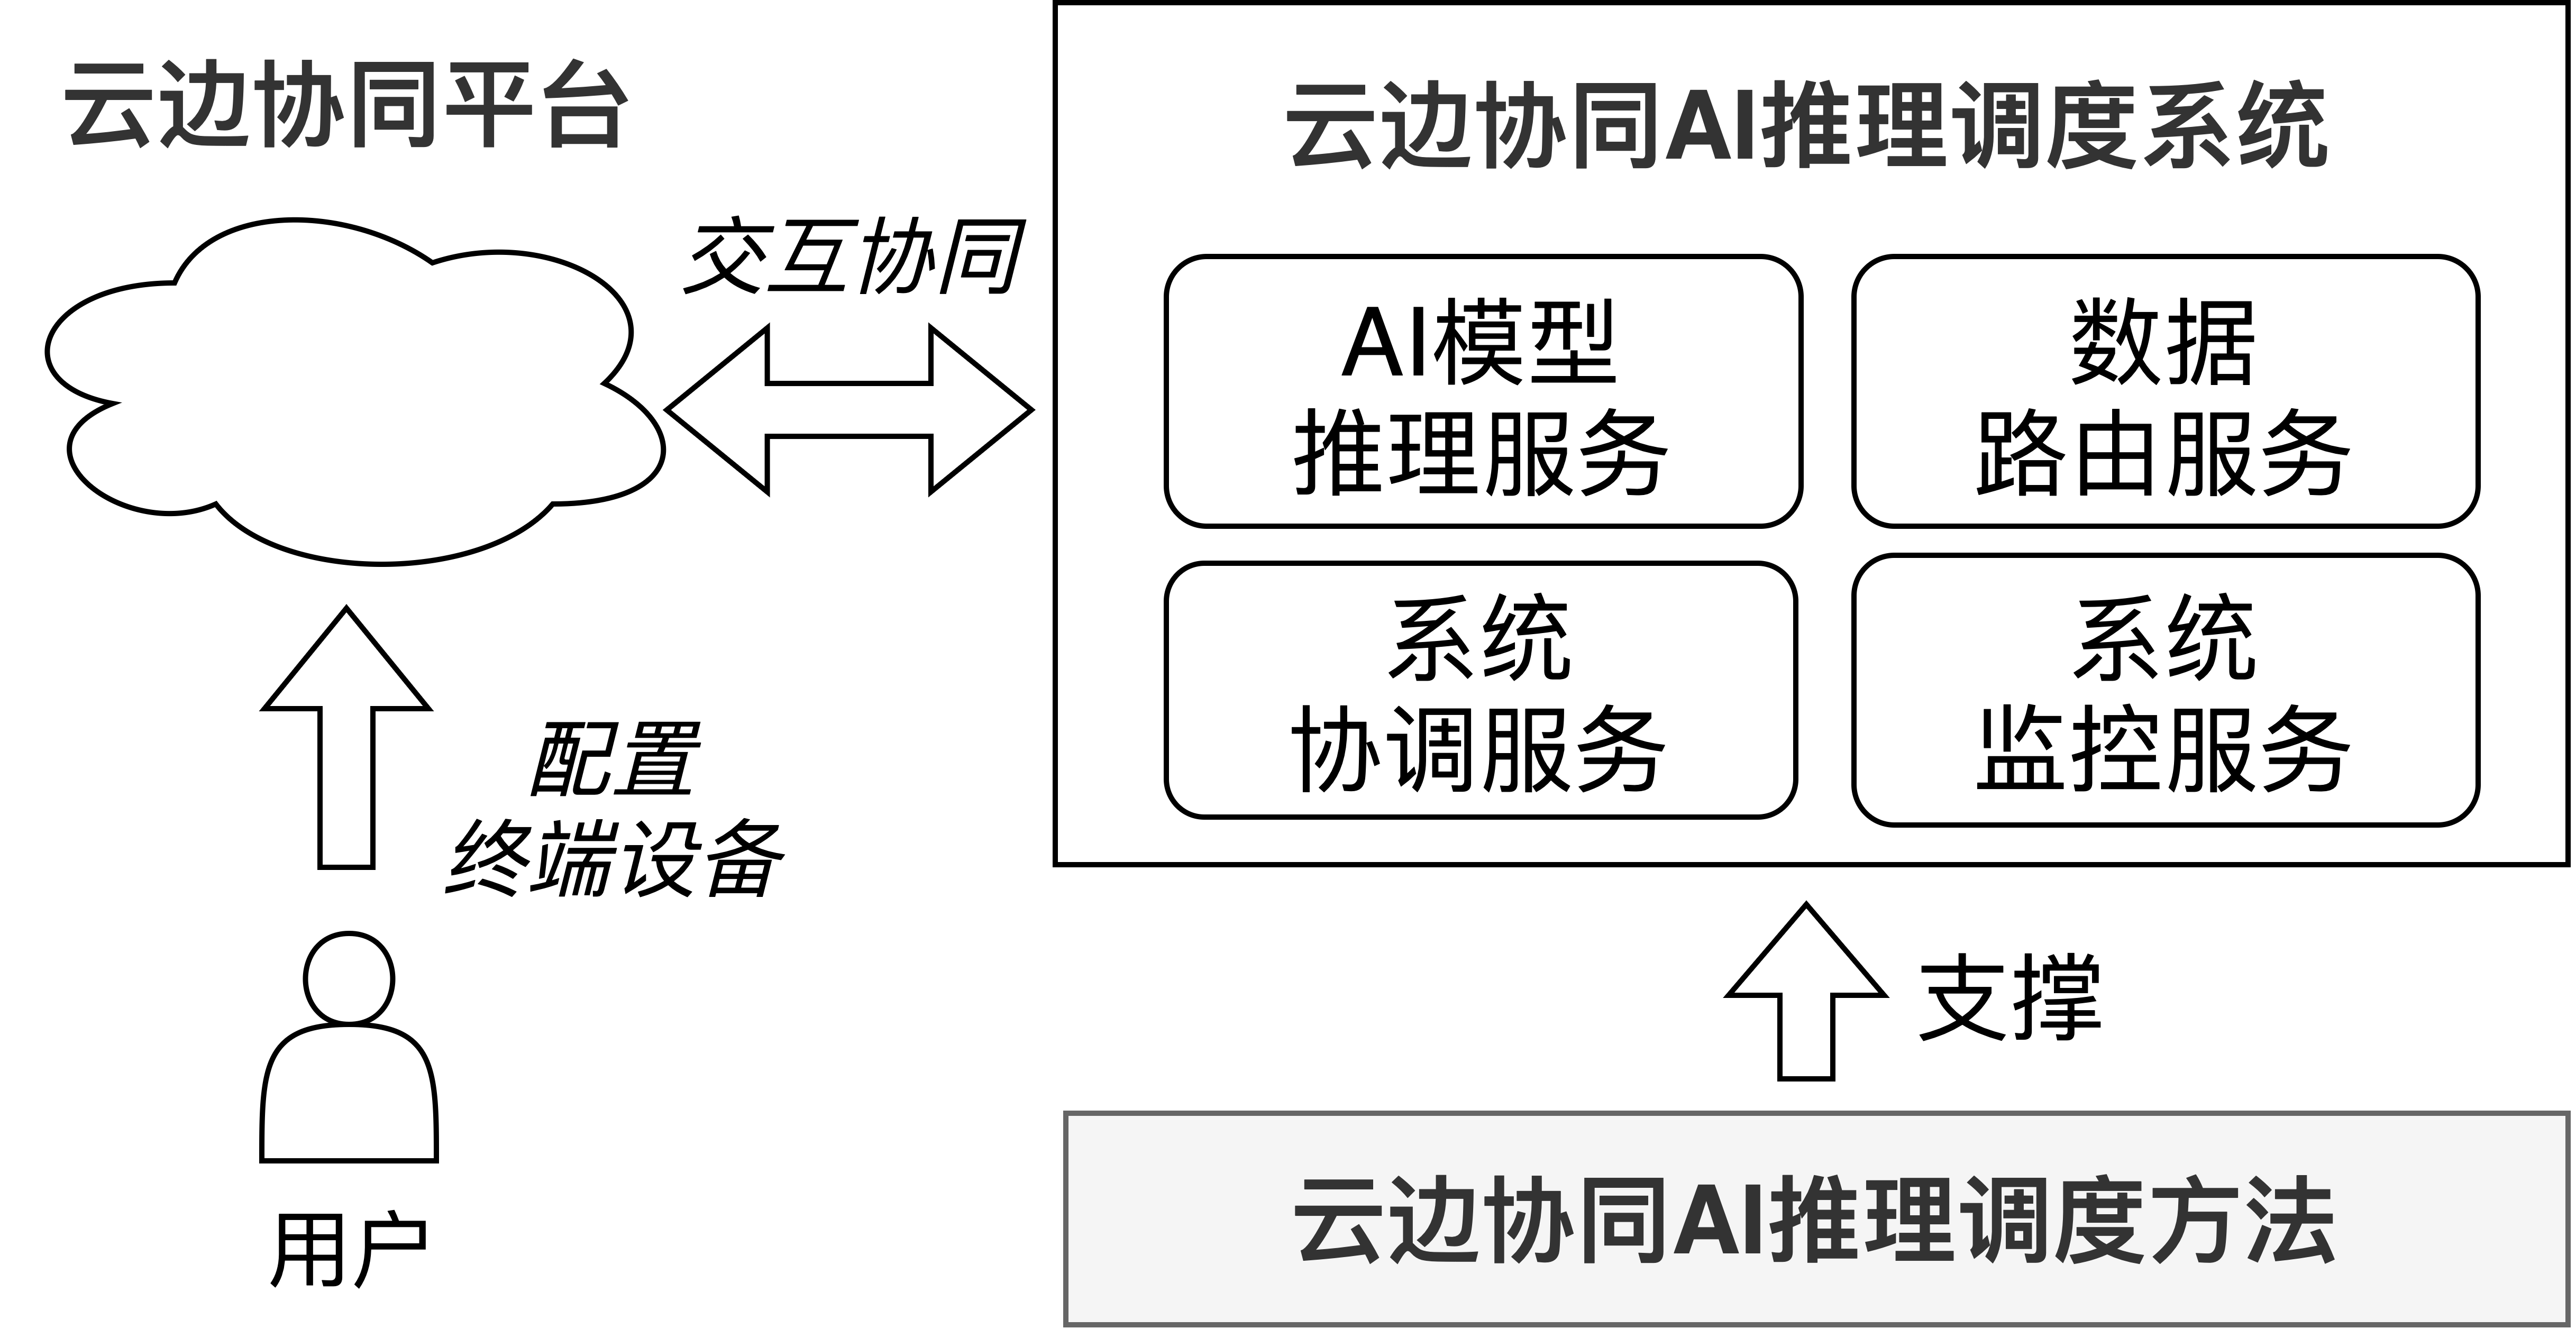
\includegraphics[width=0.7\linewidth]{pics/3-all.png}
  \caption{云边协同AI推理调度方案KEAS示意图}
  \label{fig:3-all}
\end{figure}

图\ref{fig:3-all}展示了本文提出的云边协同AI推理调度方案KEAS的整体架构。该方案涉及用户、云边协同平台、云边协同AI推理调度方法和系统等多个角色。在运行时,用户通过云边协同平台配置终端设备,这些设备会持续采集并生成流式时序数据。系统与云边协同平台保持实时交互,动态监测终端设备的状态信息,并结合边缘和云端的资源情况,动态调度流式时序数据的AI推理请求。通过边缘节点间的水平协作以及云端全局的垂直协同,该方案实现了资源的高效利用与任务的优化分配。

\begin{figure}[ht]
  \centering
  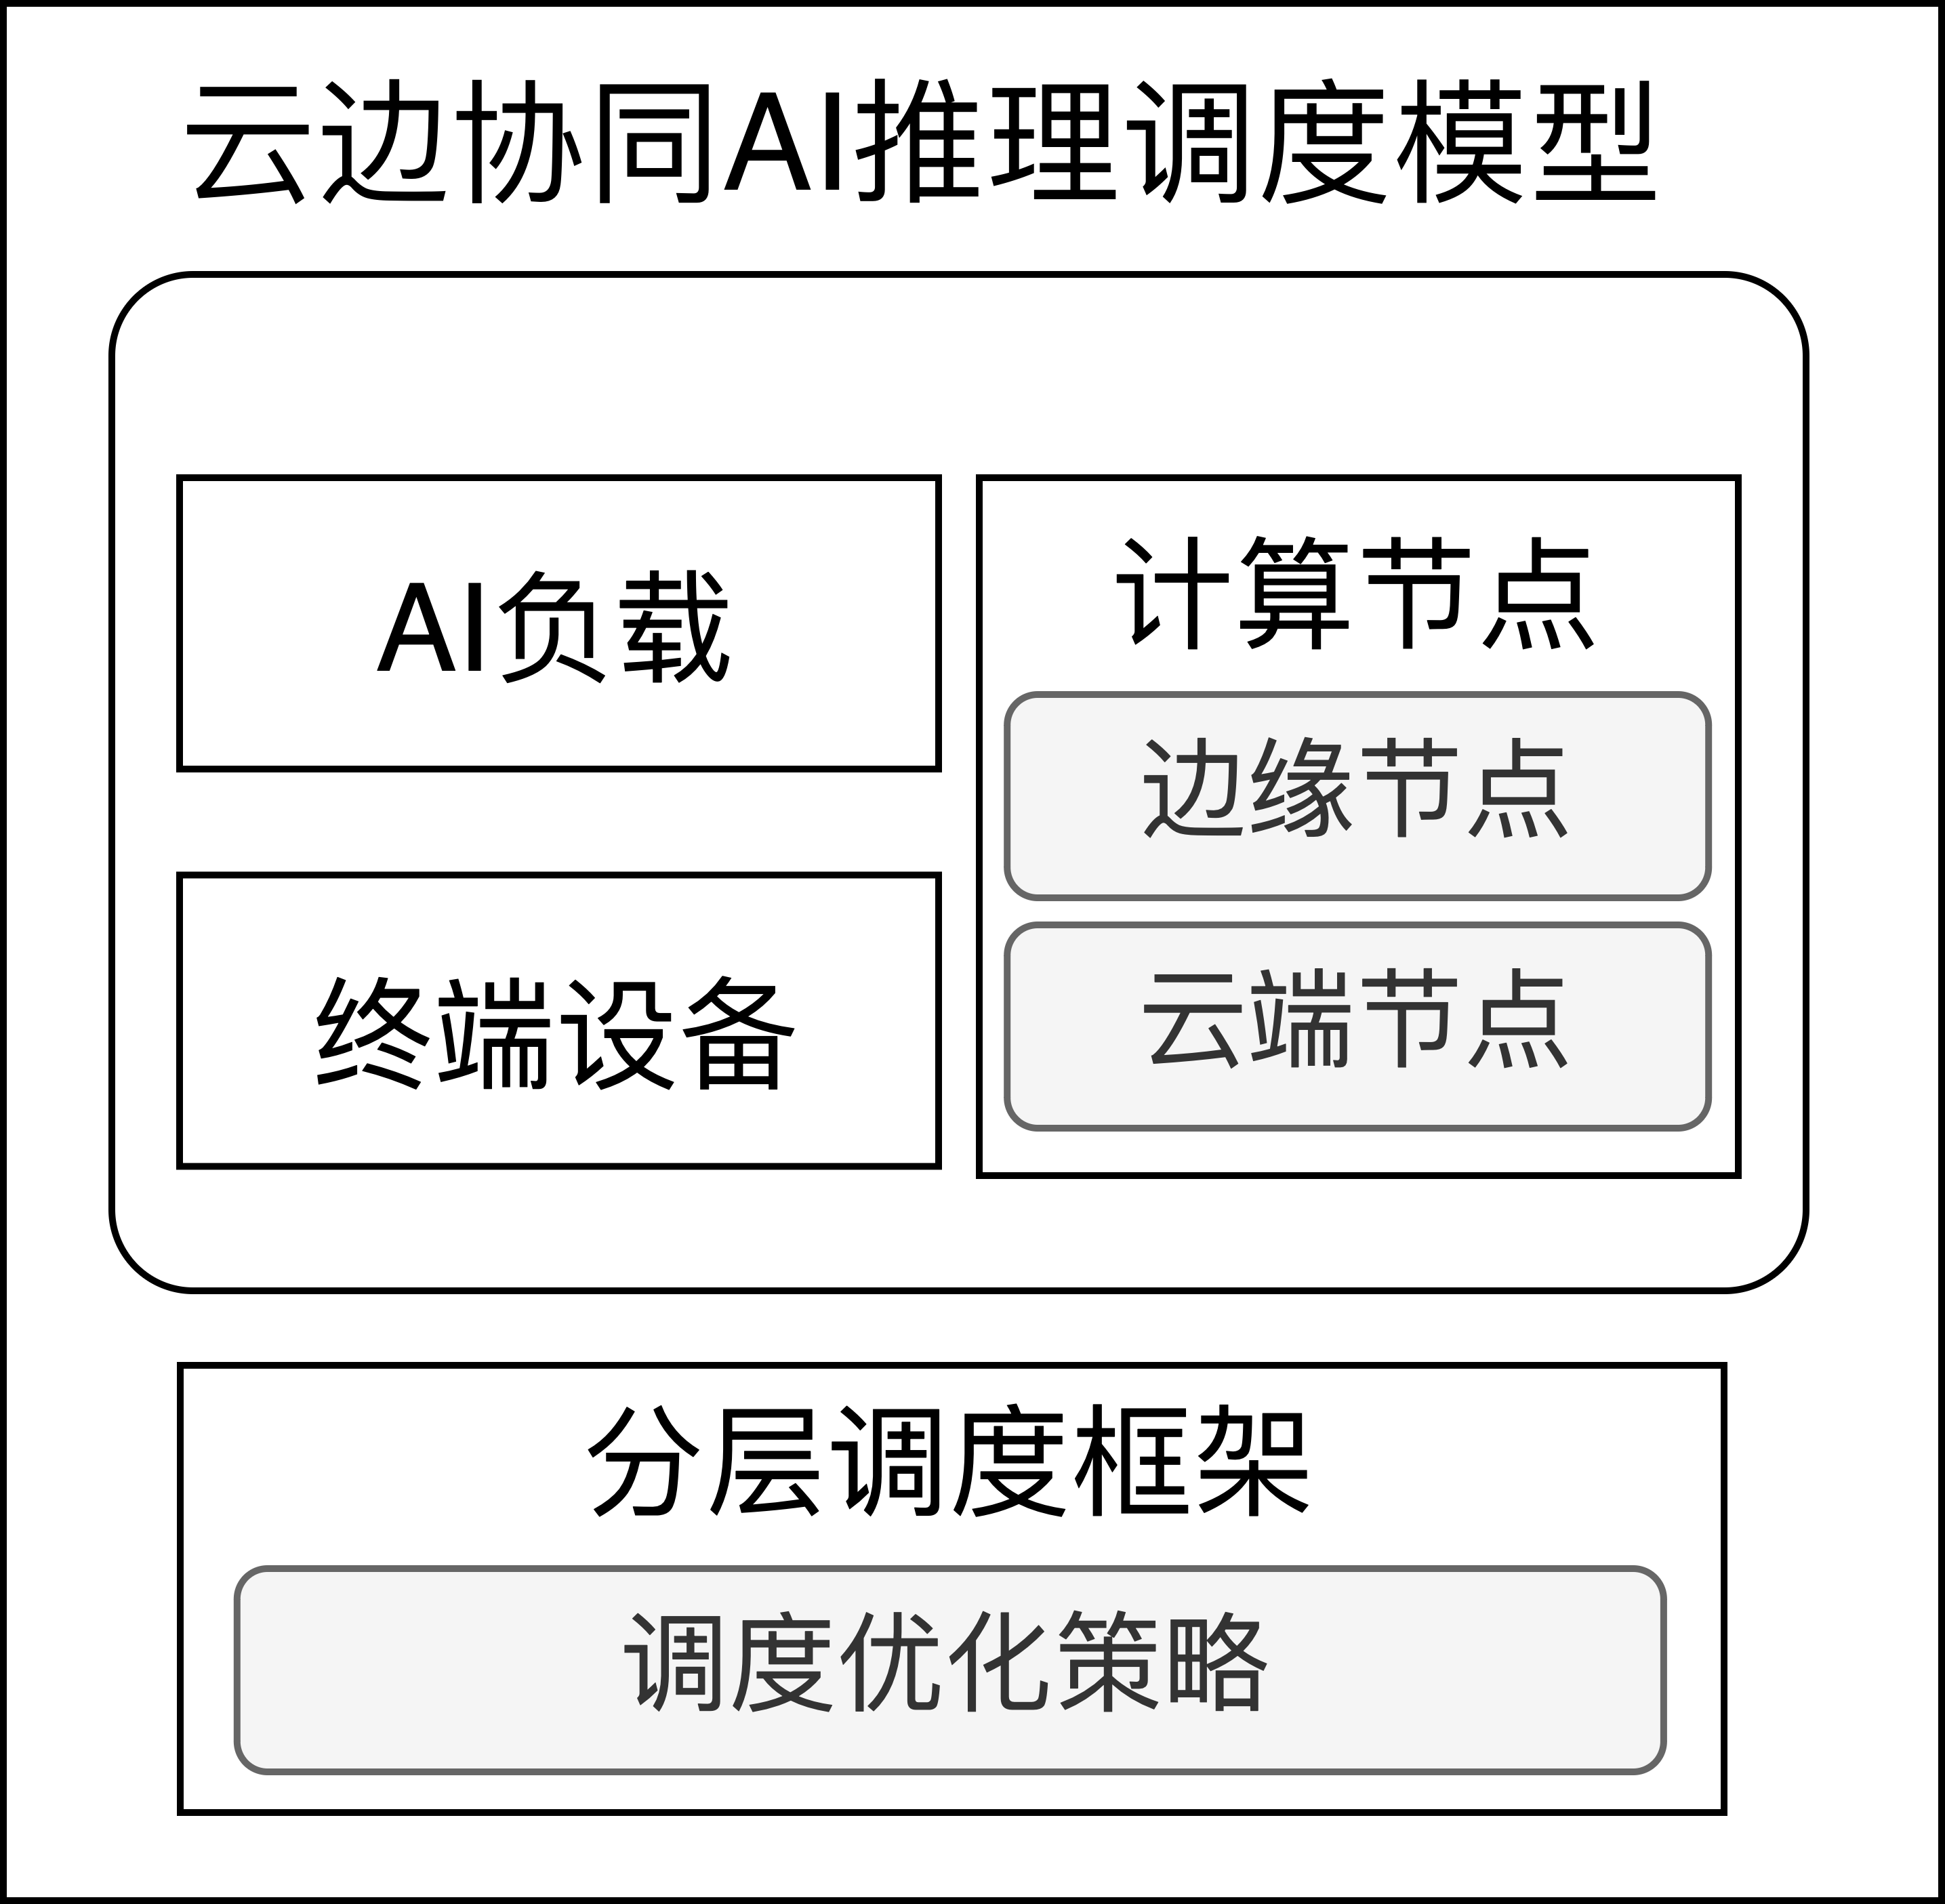
\includegraphics[width=0.8\linewidth]{pics/3-0架构.png}
  \caption{云边协同AI推理调度方法架构示意图}
  \label{fig:3-0arch}
\end{figure}

图\ref{fig:3-0arch}展示了方法的基本架构。该架构基于云边协同AI推理调度模型构建,清晰界定了云边平台的核心组件,包括终端设备、AI负载实例、计算节点、边缘集群及分层调度框架。同时,该模型详细定义了流式数据调度机制的关键要素,例如数据分流策略和各级调度器在运行时可见的状态信息等。基于此理论模型,本文提出了包含本地、边缘集群和云端全局三层结构的协同调度体系,其核心内容如下:

\begin{enumerate}
    \item \textbf{云边协同AI推理调度模型}:本文构建了形式化的云边协同AI推理调度模型,系统定义了终端设备、AI负载实例、计算节点等核心组件及其交互机制。通过引入计算队列状态感知和数据流驱动的动态调度框架,建立了覆盖边缘节点、集群到云端的多层级优化模型,为分层调度策略的设计奠定了理论基础。
    \item \textbf{云边协同AI推理分层调度策略}:本文提出三级协同调度架构。其中,本地调度策略以节点级资源最优分配为目标,通过动态调整分流比例优先保障直连设备服务质量,最小化跨节点传输开销;边缘集群调度策略在集群维度实现负载均衡,通过时延敏感度感知机制优化任务分发路径,降低集群内部协作时延;云端全局调度策略构建跨域资源协调机制,采用多目标优化模型平衡广域网带宽消耗与端到端处理时延,实现全局资源的最优配置。
    \item \textbf{云边协同AI推理分层调度优化算法}:针对多层级调度需求设计差异化优化算法。其中,本地调度采用基于优先级的贪心算法,通过单次数据量排序与弹性容量分配实现资源高效利用;边缘集群调度结合时延敏感度感知机制,构建多维度优先级队列,确保在满足时延约束的同时最大化集群内部资源利用率;云端全局调度引入随机权重帕累托优化,通过自适应权重采样与最短任务优先策略,在多项式时间复杂度内逼近多目标最优解。
\end{enumerate}

\section{云边协同AI推理调度模型}

\subsection{模型定义}

云边协同框架设计理念的核心在于实现跨层级资源的动态协同与优化调度,并在此基础上提供灵活的终端设备接入能力。现有框架通常通过抽象层屏蔽底层硬件差异,为异构设备提供标准化的接入接口。例如,KubeEdge\cite{xiong2018extend}通过设备孪生(Device Twin)技术建立物理设备的数字镜像,支持基于标准MQTT协议接入工业传感器、智能摄像头等终端设备,其双向同步机制可保证设备状态与云端视图的一致性;Tango\cite{bagchi2017tango}则提出分层设备管理模型,通过边缘代理层(Edge Proxy)对Modbus、CAN总线等工业协议进行转换,为低功耗嵌入式设备提供资源虚拟化接口。若缺乏此类模块,开发人员则需自行实现设备协议解析、数据格式转换等底层适配逻辑,完成设备管理器的设计,才能读取相关数据。

\begin{figure}[h]
  \centering
  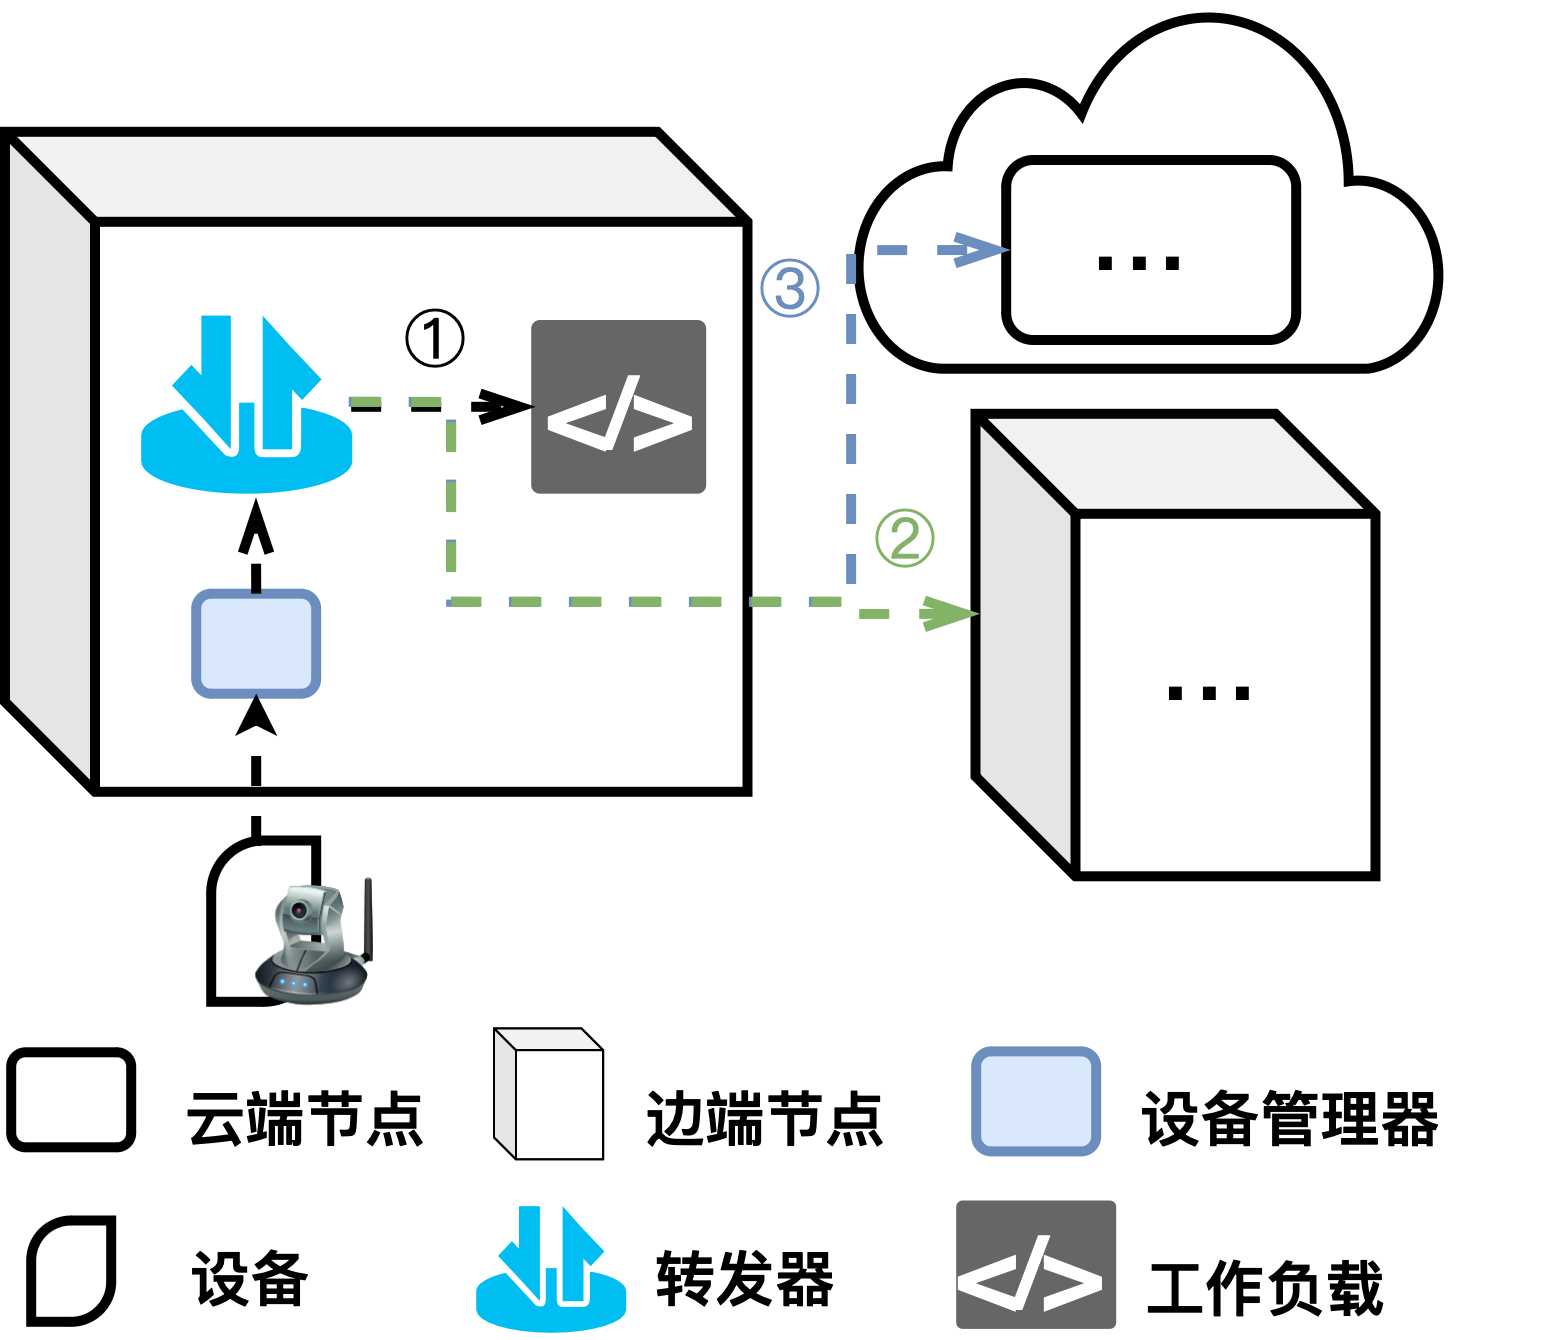
\includegraphics[width=0.5\linewidth]{pics/3-1流处理.png}
  \caption{流式数据调度与多级协作示意图}
  \label{fig:3-1flow}
\end{figure}

设备终端产生的时序数据通常需要实时处理,流处理范式因其高效性和灵活性成为云边协同框架中的关键技术之一\cite{de2018distributed,wang2020edge}。如图\ref{fig:3-1flow}所示,云边平台可根据负载状态,对于流式时序数据实现调度决策,可以在本地边缘节点直接执行,或者转发至边缘其他节点实现水平方向协作,亦可依托云端全局视图实现云边节点间跨层级的垂直方向协作。目前,部分边端流处理框架已初步支持轻量级数据过滤与转发功能。例如,Kuiper\cite{ekuiper}通过SQL-like语法定义数据过滤规则,能够对原始数据进行实时过滤与简单转换,并将结果转发至其他节点,但尚未集成智能化的动态调度决策机制。这些引擎主要面向基于阈值的轻量级计算任务,尽管部分框架尝试适配AI推理功能,但尚未充分解决云边异构化环境下AI推理任务的部署问题,缺乏对深度学习框架版本冲突的兼容性保障以及跨架构硬件适配机制。

\begin{figure}[h]
  \centering
  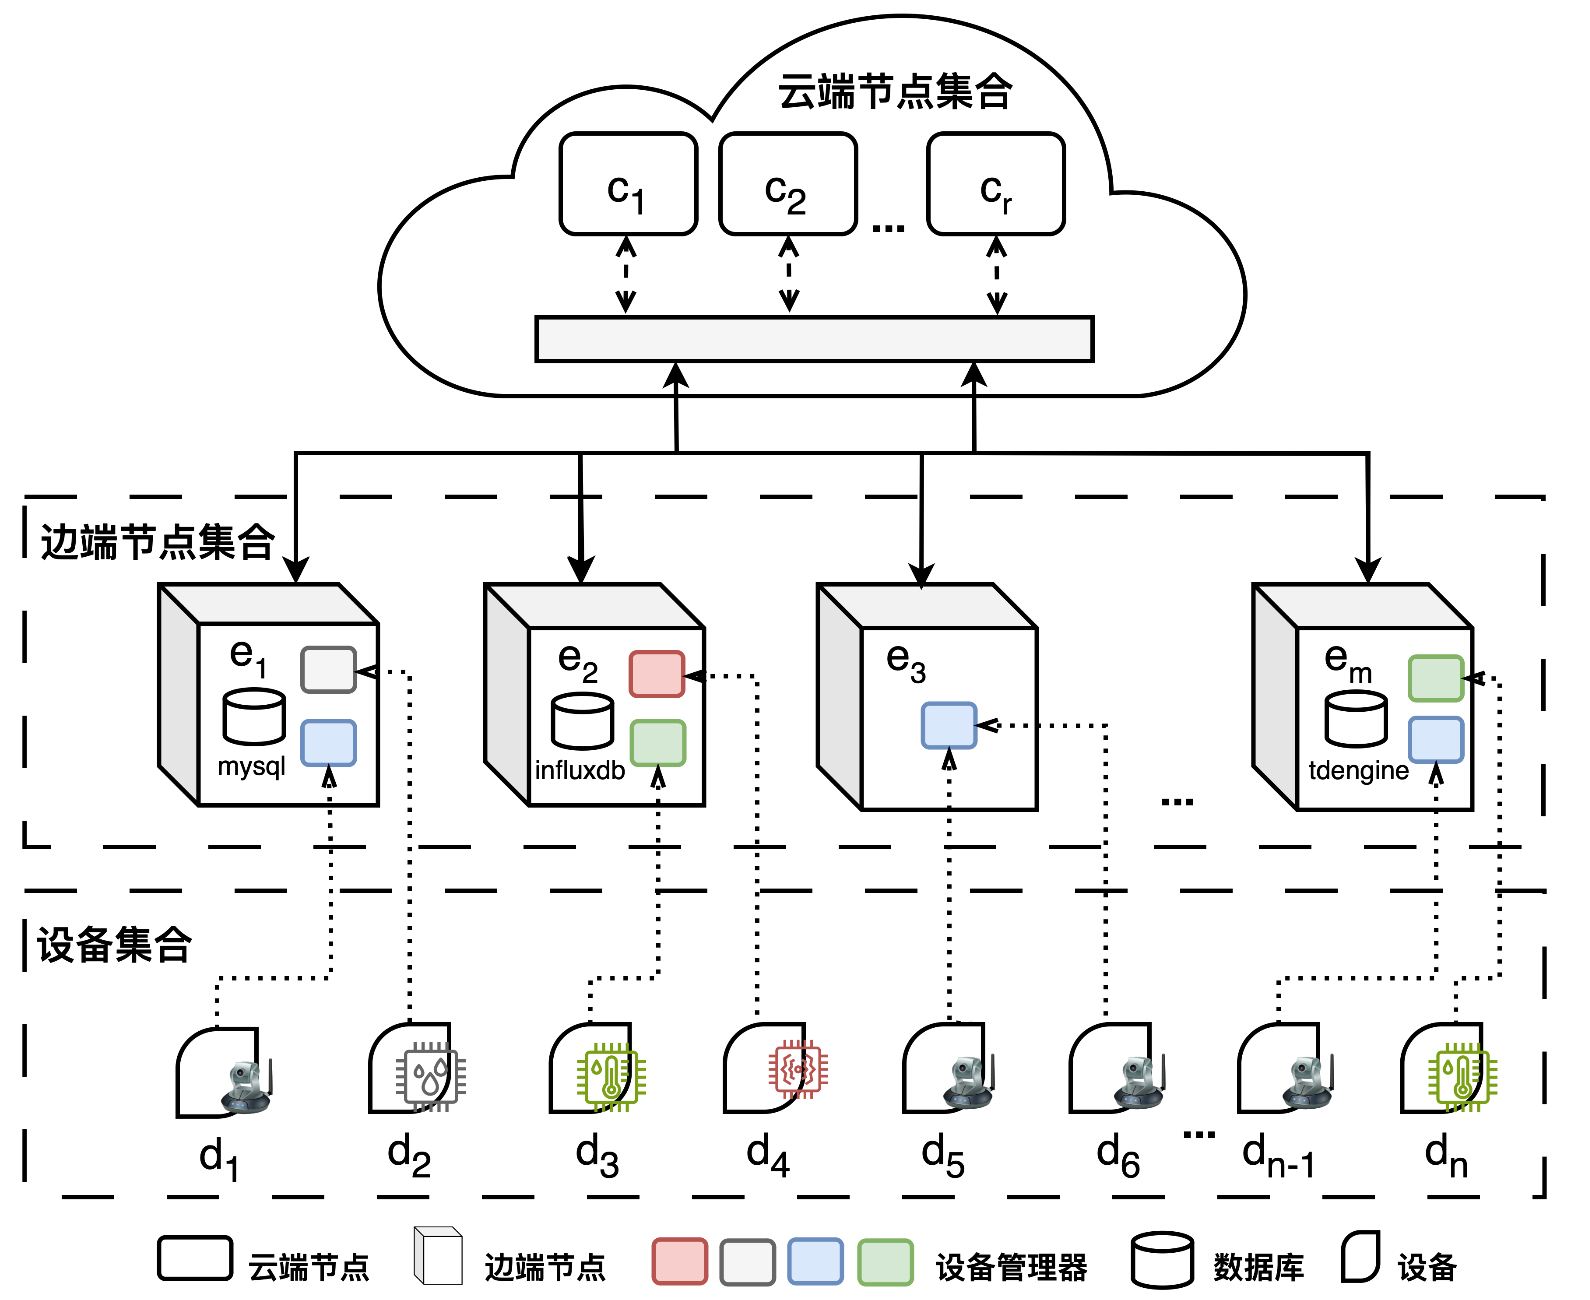
\includegraphics[width=0.8\linewidth]{pics/3-2模型架构.png}
  \caption{云边平台的分层集群拓扑架构}
  \label{fig:3-2model}
\end{figure}

在云边架构中若直接建立云端与所有边缘节点的全连接通信,云端与边缘节点之间交换的元数据(如任务状态同步、心跳检测)将随着节点数量的增加呈指数级增长,从而显著降低系统性能。例如,在包含 $N$ 个边缘节点的系统中,云端需维护 $O(N^2)$ 规模的元数据交换链路,这不仅大幅增加了网络负载,还导致带宽利用率显著下降,进而影响整体系统的运行效率。为解决这一问题,本文引入边缘集群集合作为中间抽象层,如图\ref{fig:3-2model}所示。通过将边缘节点划分为若干集群,元数据交换复杂度从$O(N^2)$降至$O(p^2)$(其中$p \ll N$为集群数量)。此外,云边平台可优先在集群内部完成服务发现与负载均衡,仅当局部资源不足时触发跨集群或云端调度,这种分级调度策略不仅降低了云边交互频率,还减少了因全局协调带来的额外开销,从而提高了系统的响应速度和资源利用率。

针对上述架构特征与技术挑战,本文提出了云边协同AI推理调度模型,旨在系统性地解决云边环境中的AI推理任务挑战。该模型通过抽象任务特征与系统约束,构建统一的调度框架以支持多样化AI应用场景。其核心目标包括:优化AI负载在云边节点间的协同调度,实现容器化AI模型的自适应部署,兼容多种深度学习框架与硬件架构,并通过实时资源监控确保任务可靠性。

下面给出云边协同AI推理调度模型的形式化定义:

\paragraph{定义3.1 (云边协同AI推理调度模型)}云边端协同 AI 负载调度模型可表示为一个7元组:

\[
\mathcal{M} = (\mathcal{D}, \mathcal{E}, \mathcal{B}, \mathcal{C}, \mathcal{L}, \mathcal{N}, \mathcal{S})
\]

其中:

\begin{itemize}
    \item $\mathcal{D} = \{d_i\}_{i=1}^n$ 表示终端设备集合,其中每个终端设备$d_i$用于物联网数据采集,具体定义详见定义3.4。
    \item $\mathcal{E} = \{e_j\}_{j=1}^m$ 表示边缘节点集合,每个节点$e_j$具有有限计算资源,部署在网络边缘靠近终端设备的位置,具有低时延响应能力。
    \item $\mathcal{B} = \{B_k\}_{k=1}^p$ 表示边缘集群集合,其中每个集群$B_k$由边缘节点子集 $\mathcal{E}_k \subseteq \mathcal{E}$ 组成,通过低时延、高带宽的内部网络互连,具体定义详见定义3.8。
    \item $\mathcal{C} = \{c_q\}_{q=1}^r$ 表示云端节点集合,每个节点$c_q$配备高性能计算资源,适用于计算密集的大规模AI推理或模型训练。
    \item $\mathcal{L} = \{\ell_s\}_{s=1}^u$ 表示AI负载实例集合,其中每个AI负载实例$\ell_s$负责处理终端设备产生的实时流数据并执行推理任务,具体定义详见定义3.5。
    \item $\mathcal{N} = (\mathcal{W}^{\mathrm{ce}}, \mathcal{W}^{\mathrm{ee}})$ 表示分层网络拓扑,其中$\mathcal{W}^{\mathrm{ce}} = (\Psi^{\mathrm{ce}}, \Gamma^{\mathrm{ce}})$表征云边传输通道质量,时延矩阵 $\Psi^{\mathrm{ce}} = [\psi^{\mathrm{ce}}_{kq}] \in \mathbb{R}^{p \times r}$ 描述边缘集群 $B_k$ 至云节点 $c_q$ 的单向传输时延,带宽矩阵 $\Gamma^{\mathrm{ce}} = [\gamma^{\mathrm{ce}}_{kq}] \in \mathbb{R}^{p \times r}$ 表征对应链路的有效带宽;$\mathcal{W}^{\mathrm{ee}} = (\Psi^{\mathrm{ee}}, \Gamma^{\mathrm{ee}})$描述边缘层互联拓扑,时延矩阵 $\Psi^{\mathrm{ee}} = [\psi^{\mathrm{ee}}_{kl}] \in \mathbb{R}^{p \times p}$ 记录集群 $B_k$ 与 $B_l$ 间通信时延,带宽矩阵 $\Gamma^{\mathrm{ee}} = [\gamma^{\mathrm{ee}}_{kl}] \in \mathbb{R}^{p \times p}$ 表示跨集群通信带宽。
    \item $\mathcal{S}$ 表示分层调度框架,负责将设备产生的流式数据动态路由至适配的AI负载实例,具体定义详见定义3.9。
\end{itemize}

为了更清晰地描述模型的动态运行特性,本文将云边平台的运行时间划分为一系列等长时间窗 $\{t_\omega\}_{\omega=1}^\infty$。其中,第 $\omega$ 个调度时间窗定义为 $t_\omega = [\tau_\omega, \tau_\omega + \Delta t)$,$\Delta t$ 表示时间窗的长度参数。在此基础上,后续章节将进一步展开对终端设备、云边环境中的 AI 负载、边缘集群以及云边协同调度机制的详细分析。

\subsubsection{终端设备}

在物联网架构下,终端设备作为数据采集的核心单元,其行为特性可从静态属性和动态数据采集两个维度进行刻画。静态属性描述了设备的固有能力与接口规范,这些属性在设备设计阶段确定且不可更改;而动态数据采集则关注设备在运行时的数据生成过程,包括采样频率、数据传输速率等,这些特性通常由外部调度策略或事件触发机制动态调整。为了更好地形式化这两种特性,本文引入了设备原型和设备管理器的概念。

设备原型用于抽象终端设备的静态属性及其相关的通信协议,提供设备的基本描述信息。每个设备原型的静态属性展现出显著的类型特异性,这种特异性源于不同设备在功能设计和物理实现上的差异。例如,视觉设备的静态属性通常包括成像分辨率、色彩位深度、压缩算法标识及总线配置等量化参数,而温度传感器则包含量程范围、测量精度等物理特性参数。这些静态属性不仅是设备基础能力的核心表征,还为数据量计算提供了关键参数。以视觉设备为例,其单帧数据量可通过分辨率与位深度的乘积进行初步估算,并结合压缩率修正得出精确值。

\paragraph{定义3.2 (设备原型)} 设备原型$\tau_\beta \in \mathcal{T}$可表示为一个 3 元组:
\[
\tau_\beta = (\Phi_\beta,\, \Omega_\beta,\, \varsigma_\beta)
\]
其中:
\begin{itemize}
    \item $\Phi_\beta = (X^{(k)}_\beta)_{k=1}^{\zeta}$ 表示静态属性集合($\zeta \in \mathbb{N}^+$为属性维度),表征设备的物理特性。
    \item $\Omega_\beta \in \mathbb{Z}^+$表示通信协议标识符,通过映射表$\chi: \mathbb{Z}^+ \to \mathcal{P}$对应具体协议实现。
    \item $\varsigma_\beta \in \mathbb{R}^+$表示单次数据采集量,通过标准化转换函数计算:
        \[
        \varsigma_\beta = \varphi(\Phi_\beta) = \prod_{k=1}^{\zeta} f_k(X^{(k)}_\beta)
        \]
        其中$f_k: \mathcal{P} \to \mathbb{R}^+$为预定义的属性量化函数。
\end{itemize}

为简化论述,本文假设初始场景下所有终端设备均基于单一设备原型 $\tau_\beta$ 采集数据,该假设通过服务发现机制扩展至多设备原型场景。设备管理器则负责封装动态数据采集逻辑,包括采集策略函数和事件驱动触发机制。采集策略函数是由系统设计者或上层应用开发者定义的一系列规则,用于指导终端设备在运行时如何生成和传输数据;而事件驱动触发机制是一种更加灵活的数据采集方式,其核心思想是通过外部事件或条件的变化来触发动态数据采集行为。

\paragraph{定义3.3 (设备管理器)} 设备管理器$\eta_\beta \in \mathcal{H}$可表示为一个 2 元组:
\[
\eta_\beta = (\xi_\beta,\, \Upsilon_\beta)
\]
其中:
\begin{itemize}
    \item $\xi_\beta$ 表示采集策略函数,$\xi_\beta(t)$ 表示当前时刻$t$的瞬时采集频率,需满足Lipschitz连续条件:
        \[
        \exists K_\beta > 0,\ \forall t_1, t_2 \in \mathbb{R},\ |\xi_\beta(t_2) - \xi_\beta(t_1)| \leq K_\beta |t_2 - t_1|
        \]
        其中$K_\beta$表示设备物理特性决定的最大调节速率。
    \item $\Upsilon_\beta = \{(\epsilon_\theta, \kappa_\theta)\}_{\theta=1}^{\iota}$ 为事件驱动触发器集合,其中每个元素由事件类型$\epsilon_\theta \in \mathbb{X}$与触发条件函数$\kappa_\theta: \mathbb{R}^+ \to \{0,1\}$构成。其中$\mathbb{X}$为预定义的事件类型枚举集,$\kappa_\theta(t)=1$表示事件$\epsilon_\theta$在时刻$t$被触发,此时将激活突发数据采集。
\end{itemize}

结合上述的设备原型和设备管理器的定义,可以进一步形式化终端设备的行为。终端设备在运行时通过设备原型中的单次数据采集量$\sigma_\alpha$与设备管理器中的动态采集策略$\xi_\beta(t)$相结合,计算出单位时间内的数据生成量。此外,事件驱动触发机制会根据特定事件的发生动态调整数据采集频率或模式,从而影响整体数据生成量。例如,对于视觉设备,单位时间内的数据生成量不仅取决于单帧数据量与瞬时频率的乘积,还需考虑由事件触发导致的突发数据流。

下面给出终端设备的形式化定义:

\paragraph{定义3.4 (终端设备)} 终端设备$d_i \in \mathcal{D}$可表示为一个 2 元组:
\[
d_i = (\tau_\beta,\, \eta_\beta)
\]
其中:
\begin{itemize}
    \item $\tau_\beta \in \mathcal{T}$表示设备原型,具体定义详见定义3.2。
    \item $\eta_\beta \in \mathcal{H}$表示设备管理器,具体定义详见定义3.3。
\end{itemize}

设备原型$\tau_\beta$与设备管理器$\eta_\beta$之间形成映射$\vartheta(\tau_\beta) = \eta_\beta$。该映射确保每个设备原型对应唯一设备管理器,从而形成完整的设备行为描述。终端设备$d_i$的瞬时数据采集频率$g_i(t)$的表达式为:

\begin{equation}
g_i(t) = \underbrace{\xi_\beta(t)}_{\text{采集策略}} + \underbrace{\sum_{\theta=1}^{\iota} \mathbb{I}_{\{\kappa_\theta(t)=1\}}}_{\text{事件驱动}}
\end{equation}

其中$\xi_i(t)$表示由采集策略函数决定的瞬时采样频率,而$\sum \mathbb{I}_{\{\kappa_\theta(t)=1\}}$则刻画了事件驱动触发机制对采样频率的动态调整。进一步地,终端设备$d_i$的瞬时数据采集流量$G_i(t)$由瞬时数据采集频率$g_i(t)$与单次采集量$\varsigma_\beta$共同决定,具体表达式为:

\begin{equation}
G_i(t) = g_i(t) \cdot \varsigma_\beta
\end{equation}

根据终端设备的定义,可以完整抽象设备的数据采集过程,如图\ref{fig:3-3device}所示。首先,开发人员将设备原型$\tau_\beta \in \mathcal{T}$注册至云边平台,在此过程中,云边平台通过解析设备原型的静态属性集合 $\Phi_\beta$ 和通信协议标识符 $\Omega_\beta$,提取出设备的关键能力描述,并自动生成对应的设备管理器 $\eta_\beta$。利用预定义的标准化转换函数 $f_k$ 对静态属性进行量化后,可计算得到每次数据传输的具体量 $\varsigma_\beta = \varphi(\Phi_\beta)$。在此基础上,设备管理器进一步整合动态采集策略 $\xi_\beta(t)$ 和事件驱动触发器集合 $\Upsilon_\beta$,通过实时调整瞬时采样频率或响应外部事件 $\epsilon_\theta$,以满足不同时段对设备数据采集的需求。

\begin{figure}[h]
  \centering
  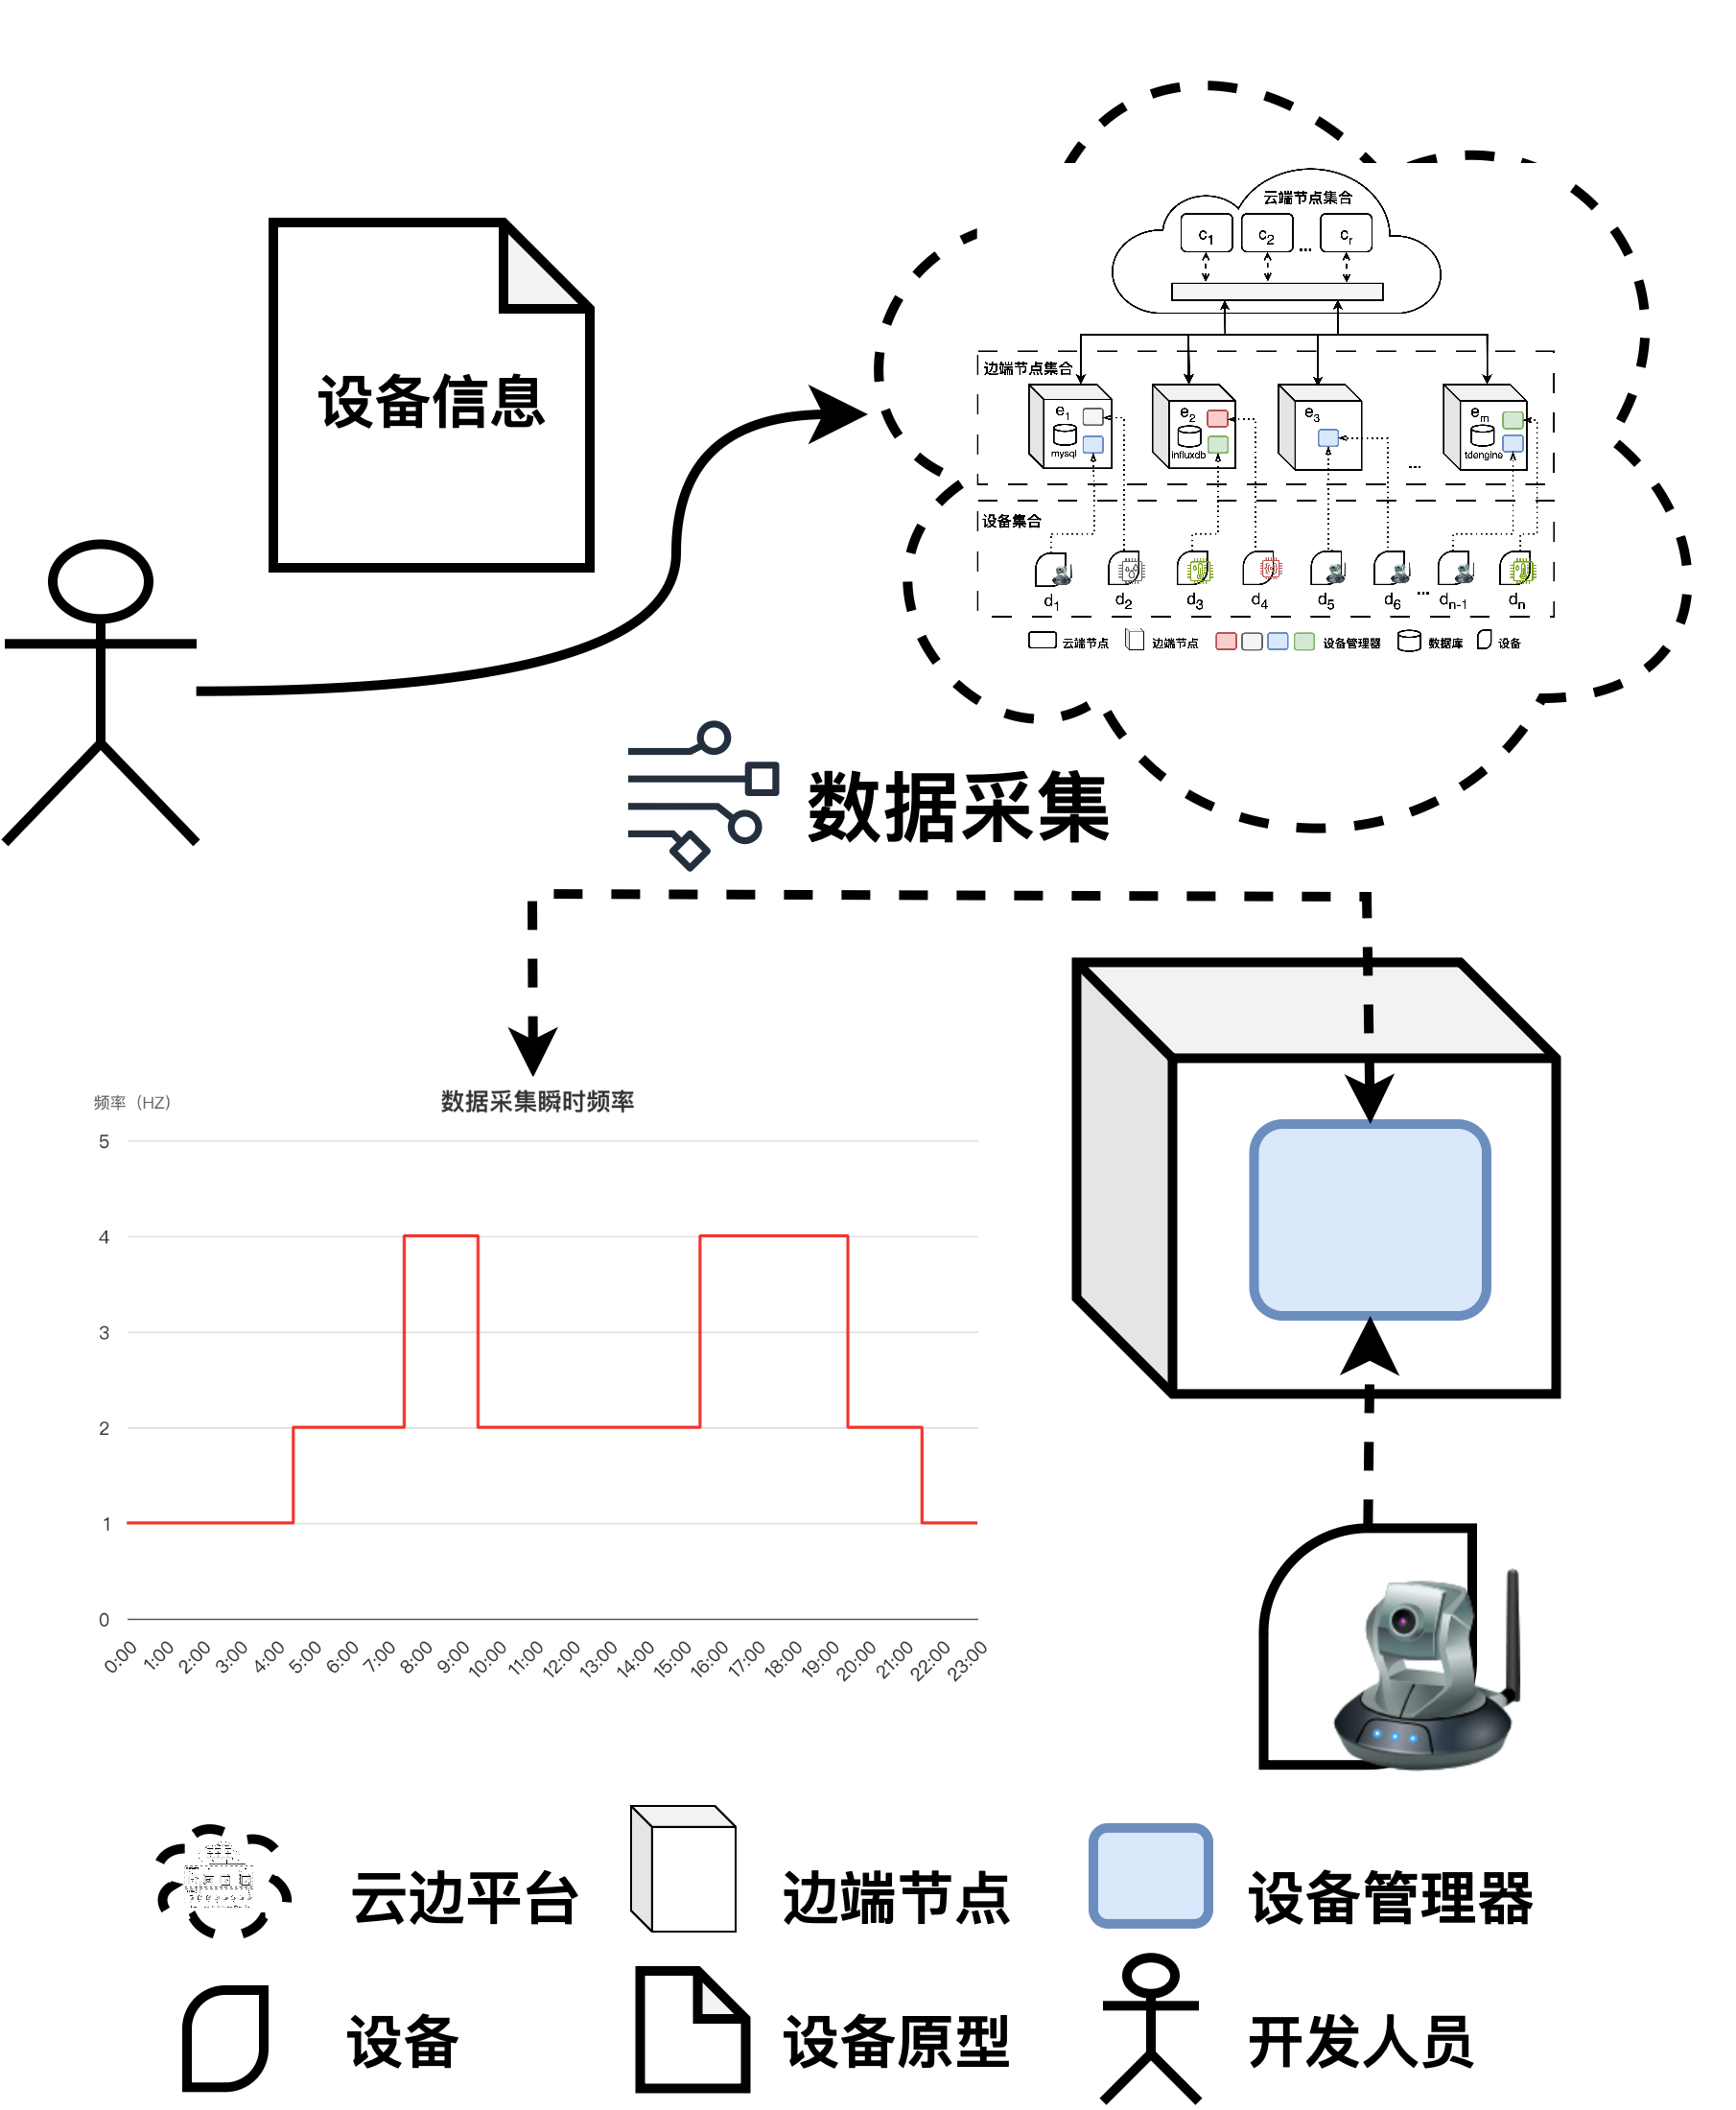
\includegraphics[width=0.55\linewidth]{pics/3-3设备模型.png}
  \caption{设备数据采集流程图}
  \label{fig:3-3device}
\end{figure}

\subsubsection{云边环境中的AI负载}

在云边协同的推理场景中,AI负载实例的核心功能是处理终端设备产生的实时流数据。终端设备(如传感器、摄像头等)持续生成大量高时效性和多样性的实时数据流。然而,这些原始数据通常需要经过预处理才能被AI负载实例有效利用。由于不同类型的终端设备生成的数据格式和特性各异,其预处理需求也各不相同。例如,视觉设备可能需要图像压缩或格式转换,而传感器数据可能需要滤波或归一化处理。如图\ref{fig:3-4aiload}所示,预处理逻辑的部署位置具有灵活性:既可以在设备管理器采集数据时实时完成,也可以在AI推理实例中进行处理。此外,云边环境中的数据转发器能够根据实际需求,选择性地传输已预处理的结构化数据或原始数据,从而在保持数据时效性的同时,为不同场景提供灵活的处理方案。

\begin{figure}[h]
  \centering
  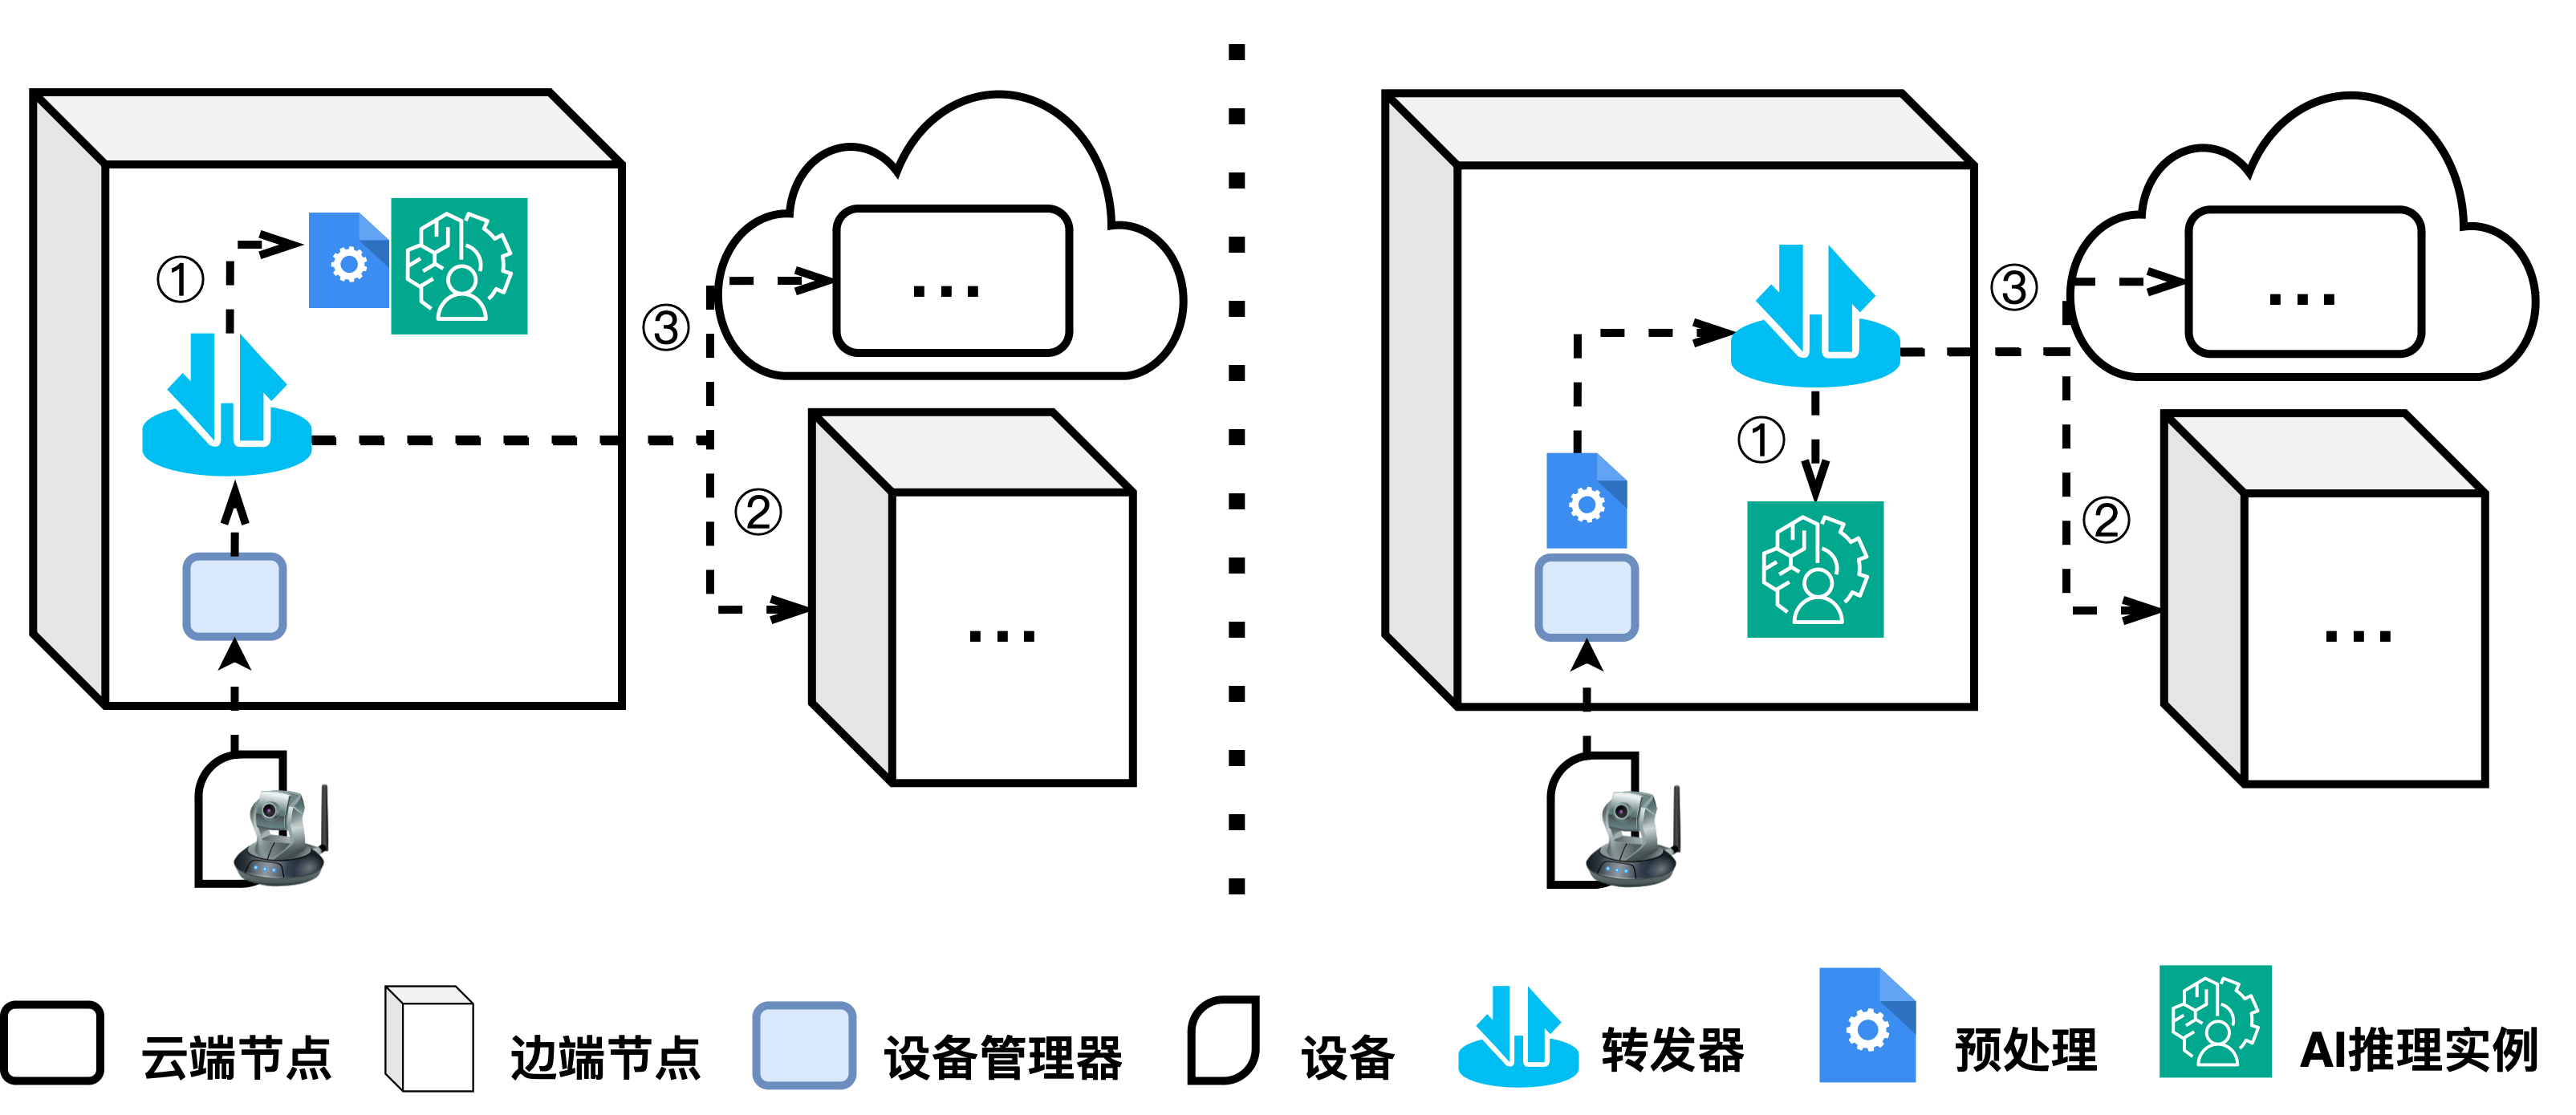
\includegraphics[width=0.9\linewidth]{pics/3-4AI负载.png}
  \caption{云边环境下AI负载的端到端处理流程}
  \label{fig:3-4aiload}
\end{figure}

当经过预处理的数据传递至AI负载实例后,推理过程即可在适配的计算节点上执行。然而,AI负载实例对不同节点的适配性存在显著差异,这主要体现在深度学习框架、硬件指令集依赖与推理资源需求等方面。首先,AI模型通常在特定框架及其版本下开发,而不同计算节点可能未安装所需的框架或版本。此外,许多框架的版本与其对硬件指令集的支持深度绑定,这种绑定关系直接影响模型的部署和运行效率。例如,当前主流框架(如TensorFlow)的最新版本通常默认启用AVX2指令集优化,以大幅提升张量运算性能。然而,在将其部署到不支持AVX2指令的边缘节点时,则需要通过重新编译框架源码或降级至兼容版本来实现正常运行。即便目标节点具备相应的硬件指令集,不同架构(如x86与ARM)对同一指令集的优化程度也可能导致运行效率的显著差异\cite{ren2019performance}。这种硬件架构的异构性要求在部署AI负载时,必须明确其对指令集和架构的具体需求。

其次,资源需求是影响AI负载适配性的另一关键因素。许多大型深度学习模型在设计之初便针对GPU等高性能加速器进行优化,依赖于GPU的大规模并行计算能力。然而,在资源受限的边缘节点上,可能缺乏GPU或其他专用加速器,导致模型无法运行或运行效率低下。同时,为了充分利用节点的计算能力,不同的AI负载实例会根据节点性能配置相应的批处理规模。例如,在高性能云端节点上可以采用较大的批处理规模以提高吞吐量,而在资源受限的边缘节点上则需降低批处理规模以避免资源过载。

上述问题表明,异构环境下的AI负载部署面临诸多挑战,包括框架兼容性、指令集支持以及资源适配性等复杂因素。为了解决这些问题,我们需要形式化定义AI负载实例的关键属性,以量化其对框架、硬件架构和资源的需求,并评估其在不同节点上的适配性。这种形式化的描述不仅有助于优化任务调度策略,还能显著提升系统在动态异构环境中的整体性能。

\paragraph{定义3.5 (AI负载实例)} AI负载实例$\ell_s \in \mathcal{L}$ 可表示为一个 5 元组:
\[
\ell_s = (\mathcal{F}_s,\, \mathcal{A}_s,\, \mathcal{R}_s,\, \gamma_s,\, \varpi_s)
\]
其中:
\begin{itemize}
    \item $\mathcal{F}_s \in \mathbb{S}$ 表示支持的深度学习框架,$\mathbb{S}$为云边平台支持的深度学习框架枚举集。
    \item $\mathcal{A}_s \subseteq \mathbb{H}$ 表示硬件架构需求集合,$\mathbb{H}$为硬件架构类型枚举集。
    \item $\mathcal{R}_s = \{r^{(k)}_s\}_{k=1}^v$ 表示资源需求向量,其中$r^{(k)}_s \in \mathbb{R}^+$对应第$k$类资源的最小需求。
    \item $\gamma_s \in \mathbb{Z}^+$ 表示批处理规模,满足$\gamma_s \leq \lfloor R_s/\delta_s \rfloor$,其中$R_s$为设备内存容量,$\delta_s$为单样本内存占用量。
    \item $\varpi_s \in \mathbb{R}^+$ 表示单次推理运算量,单位为浮点运算次数。
\end{itemize}

在明确了AI负载实例的形式化定义后,我们还需要进一步形式化计算节点的属性。这是因为计算节点的资源供给和硬件架构直接决定了AI负载实例能否成功部署和高效运行。通过形式化定义计算节点,我们可以量化节点的资源供给能力、硬件架构特性以及计算能力,从而为AI负载实例的调度提供理论依据。具体而言,计算节点集合$\mathcal{V} = \mathcal{E} \cup \mathcal{C}$涵盖边缘节点集合$\mathcal{E}$与云端节点集合$\mathcal{C}$,其中总共包含$\mu=m+r$个计算节点。

\paragraph{定义3.6 (计算节点)} 计算节点$v_j \in \mathcal{V}$ 可表示为一个 3 元组:
\[
v_j = (\rho_j,\, \alpha_j,\, \vartheta_j)
\]
其中:
\begin{itemize}
    \item $\rho_j = \{r^{(k)}_j\}_{k=1}^v$ 表示资源供给向量,其中$r^{(k)}_j \in \mathbb{R}^+$表示第$k$类资源总量。
    \item $\alpha_j \in \mathbb{H}$ 表示硬件架构,$\mathbb{H}$为硬件架构类型枚举集。
    \item $\vartheta_j \in \mathbb{R}^+$ 表示计算能力,单位为单位时间浮点运算次数(FLOPs)。
\end{itemize}

基于对AI负载实例与计算节点的形式化定义,本文构建推理时间预测函数$\Theta(\ell_s, v_j)$来量化负载实例$\ell_s$在节点$v_j$上的单次推理延迟。该函数综合考虑计算资源消耗与系统级开销,其表达式为:

\begin{equation}
\Theta_{\text{inf}}(\ell_s, v_j) = \underbrace{\frac{\varpi_s}{\vartheta_j}}_{\text{核心计算时延}} + \underbrace{\Xi(\ell_s, v_j)}_{\mathclap{\text{额外时延}}}
\end{equation}

其中$\Xi: \mathcal{L} \times \mathcal{V} \to \mathbb{R}^+ \cup \{\infty\}$表示系统级额外时延开销。

对于任意时间窗$t_\omega = [\tau_\omega, \tau_\omega + \Delta t)$,节点$v_j$可承载的AI负载实例$\ell_s$的最大吞吐量$Q(\ell_s, v_j, t_\omega)$可由下式计算:

\begin{equation}
Q(\ell_s, v_j, t_\omega) = \left\lfloor \frac{\Delta t}{\Theta(\ell_s, v_j)} \right\rfloor \cdot \gamma_s
\end{equation}

该指标$Q(\ell_s, v_j, t_\omega)$表示节点$v_j$在时间窗$t_\omega$内对负载$\ell_s$的最大服务容量,是衡量节点资源利用率和服务能力的重要参考。在实际部署过程中,这一指标由节点资源监控模块动态维护,并作为协同调度器决策过程的核心输入之一。具体而言,调度器需确保分配至节点$v_j$的负载实例$\ell_s$的请求速率不超过其最大吞吐量$Q(\ell_s, v_j, t_\omega)$,从而避免因计算资源过载而导致的排队延迟或任务失败。为了更精确地刻画节点的服务行为并动态跟踪其负载状态,本文引入计算队列的概念,用于表征节点 $v_j$ 在时间窗 $t_\omega$ 内为 AI 负载实例 $\ell_s$ 维护的服务请求列表及其容量限制。

\paragraph{定义3.7 (计算队列)} 计算队列$\mathcal{Q}_s^j(t_\omega)$可表示为一个 2 元组::
\[
\mathcal{Q}_s^j(t_\omega) = \left( \Lambda_s^j(t_\omega),\, \lambda_s^j(t_\omega) \right)
\]
其中:
\begin{itemize}
    \item $\Lambda_s^j(t_\omega) \in \mathbb{Z}^+$表示AI负载实例$\ell_s$在节点$v_j$于时间窗$t_\omega$内的最大吞吐量,可用公式$Q(\ell_s, v_j, t_\omega)$计算。
    \item $\lambda_s^j(t_\omega) \in \mathbb{N}$ 表示当前队列长度,需满足容量约束 $0 \leq \lambda_s^j(t_\omega) \leq \Lambda_s^j(t_\omega)$。
\end{itemize}

\subsubsection{边缘集群}

边缘集群是云边协同架构中的关键中间层,旨在通过分层管理降低云端与边缘节点之间的通信开销,并提升任务调度效率。如图\ref{fig:3-5edgecluster}所示,本文设计的边缘集群采用主从结构,其中主节点不仅集群协调者的角色,还能够直接参与数据处理任务,从而更高效地利用计算资源;从节点则专注于执行具体的计算任务。

\begin{figure}[h]
  \centering
  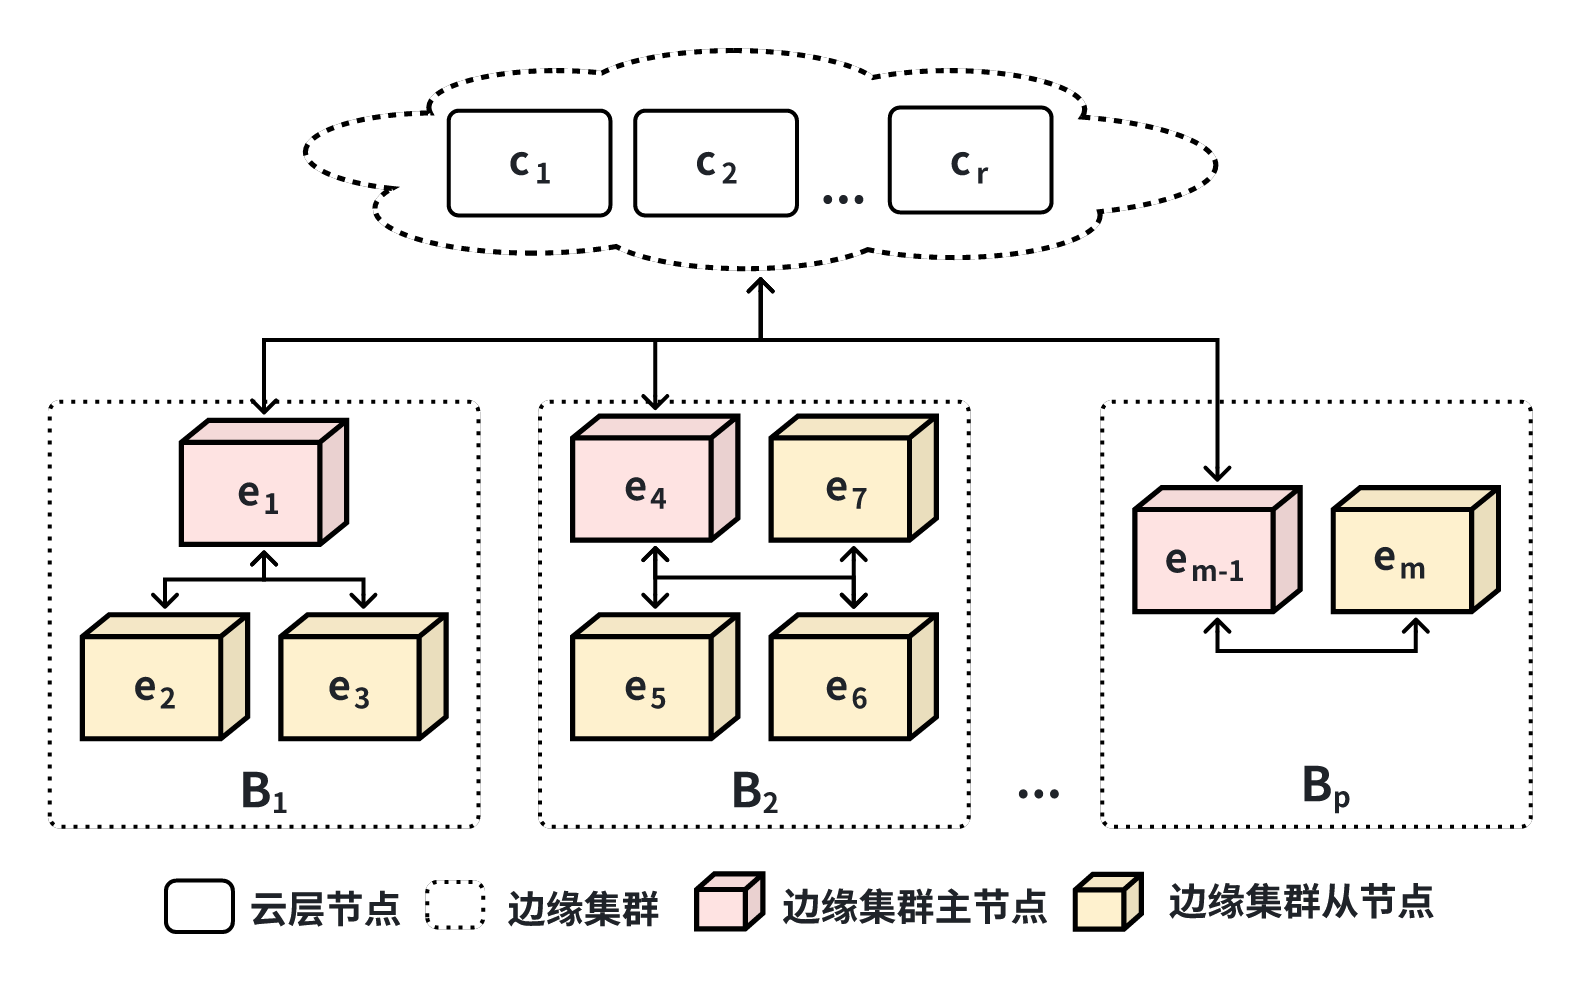
\includegraphics[width=0.8\linewidth]{pics/3-5边缘集群.png}
  \caption{主从结构的边缘集群概览}
  \label{fig:3-5edgecluster}
\end{figure}

主节点作为边缘集群的核心组件,其主要职责包括元数据管理、跨层通信以及集群内部的任务调度。首先,主节点维护并同步边缘集群的元数据,这些元数据分为两类:静态资源状态和运行状态。静态资源状态则描述了集群的固有能力,涵盖各节点的资源供给情况、计算能力;运行状态反映集群的动态行为,包括各节点负载的实时计算队列、节点健康状态等动态信息。主节点通过定期与云端通信,将上述元数据上传至云端,为云端进行全局调度决策提供依据。此外,主节点还负责集群内部的任务调度。当某个边缘节点因资源不足或故障而无法支持特定任务时,主节点会基于当前集群内部状态,在其他具备适配资源的节点中寻找最优候选者完成任务分配。

根据边缘集群的架构设计与主节点的功能特性,为了更清晰地描述边缘集群的组成结构及其运行机制,本文引入了边缘集群的形式化定义。

\paragraph{定义3.8 (边缘集群)} 边缘集群$B_k \in \mathcal{B}$可表示为一个 3 元组:
\[
B_k = (L_k, \mathcal{E}_k, \Phi_k)
\]
其中:
\begin{itemize}
    \item $L_k$表示主节点,属于计算节点集合$\mathcal{E}$的特殊元素,承担集群协调者的角色。
    \item $\mathcal{E}_k = \{e_{kj}\}_{j=1}^{m_k} \subseteq \mathcal{E}$表示隶属本集群的边缘节点集合,且$L_k \equiv e_{k1} \in \mathcal{E}_k$,即主节点$L_k$也被视为该集合中的一个节点,用$e_{k1}$表示。
    \item $\mathcal{W}_k = (\Psi_k, \Gamma_k)$ 表示内部网络拓扑参数。其中,$\Psi_k = [\psi_{jj'}^{(k)}] \in \mathbb{R}^{m_k \times m_k}$ 为时延矩阵,$\psi_{jj'}^{(k)}$表示节点$e_{kj}$到$e_{kj'}$的单向传输时延;$\Gamma_k = [\gamma_{jj'}^{(k)}] \in \mathbb{R}^{m_k \times m_k}$ 为带宽矩阵,$\gamma_{jj'}^{(k)}$表示节点$e_{kj}$到$e_{kj'}$的可用带宽
\end{itemize}

\subsubsection{云边环境下的协同调度}

在云边协同架构中,调度器的核心目标是将终端设备产生的流式数据高效地分流至适配的计算节点上进行处理。然而,这种调度面临显著挑战:边缘集群内部具备高带宽、低延时的通信特性,而边缘集群间或云边之间的通信则表现出高延时、低带宽的特点。因此,调度策略需要兼顾局部响应效率与全局资源优化,这对传统集中式调度机制提出了严峻考验。本文提出一种基于计算资源层级化管理的动态任务分配机制,旨在通过多级调度器的协作优化AI推理任务的执行效率与资源利用率。

\begin{figure}[h]
  \centering
  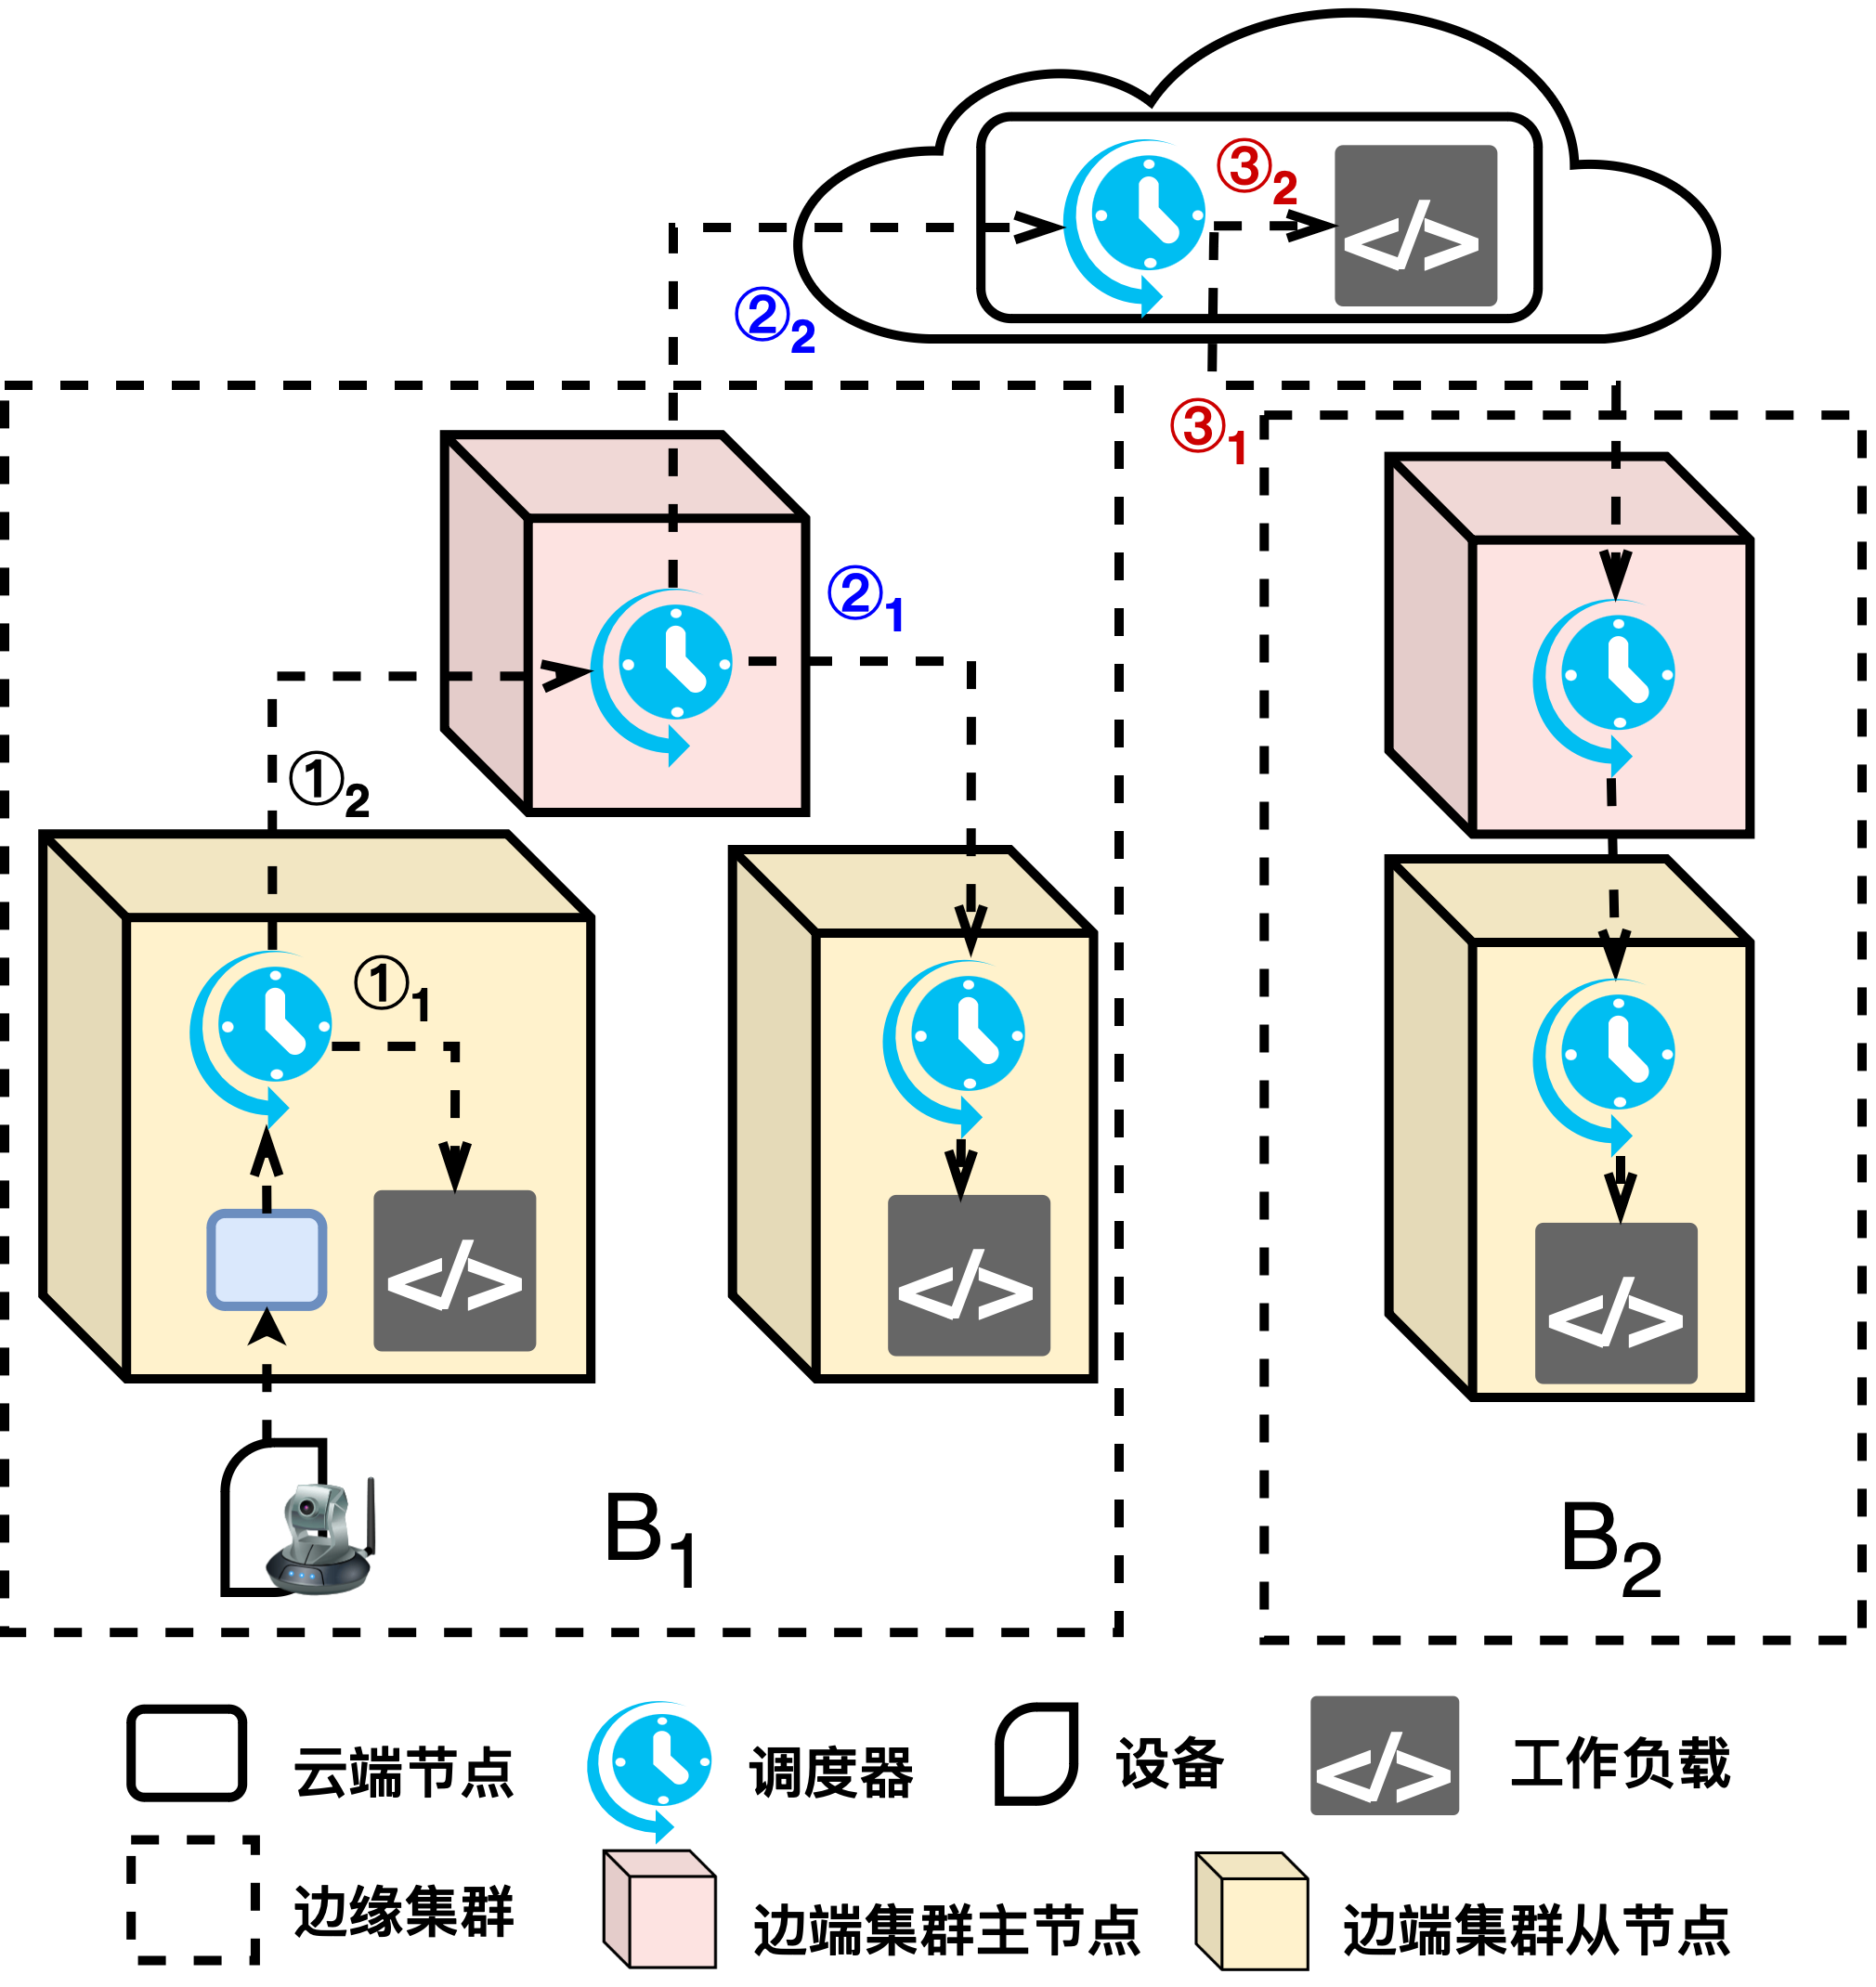
\includegraphics[width=0.6\linewidth]{pics/3-6调度器.png}
  \caption{多级调度器协作示意图}
  \label{fig:3-6scheduler}
\end{figure}

如图\ref{fig:3-6scheduler}所示,分层调度框架采用三级协同决策机制,其核心调度流程如下:当终端设备生成数据流时,框架首先尝试将终端设备产生的数据流在本地计算节点内完成处理;若本地计算节点无法满足AI负载实例 $\ell_s$ 的部署需求(例如,缺乏适配的硬件架构支持或资源供给不足),或者本地计算队列 $\mathcal{Q}_s^j(t_\omega)$ 的容量已饱和,则将任务转发至所属边缘集群进行进一步调度;若边缘集群内的所有计算队列均已达到容量上限,任务最终会被提交至云端全局调度器,以利用跨集群或云端资源实现动态分配。

\paragraph{定义3.9 (分层调度框架)} 分层调度框架$\mathcal{S}$可表示为一个 3 元组
\[
\mathcal{S} = (S_L, S_B, S_C)
\]
其中:
\begin{itemize}
    \item $S_L$表示本地调度器,负责在计算节点内部对终端设备的流处理任务进行局部调度与资源分配。
    \item $S_B$表示边缘集群调度器,用于在边缘计算集群范围内对终端设备的流处理任务进行协调性调度和优化。
    \item $S_C$表示云端全局调度器,旨在实现跨边缘与云端的全局范围内终端设备流处理任务的统一调度与资源管理。
\end{itemize}

上述分层调度框架中的每个调度器均具有独立的优化策略,这些策略在不同层级上分别关注局部资源利用率、集群范围内的负载均衡以及全局资源的最优分配。为了系统化描述各层级调度器的策略选择机制,并实现从终端设备到边缘集群再到云端的全链路协同优化,本文引入了统一的调度优化策略形式化定义。

\paragraph{定义3.10 (调度优化策略)} 调度优化策略$\mathcal{S}_{\text{opt}}(\mathcal{V}_G^κ)$可表示为一个 2 元组
\[
\mathcal{S}_{\text{opt}}(\mathcal{V}_G^κ) = (\Upsilon_{t_\omega}^κ, \Lambda_{\text{QoS}})
\]

其中:
\begin{itemize}
    \item $\Upsilon_{t_\omega}^κ = (\mathcal{Q}_{t_\omega}^κ, \mathcal{G}_{t_\omega}^κ)$ 表示层次化运行时状态,可以对应节点级、集群级和全局级状态,定义详见定义3.13。
    \item $\Lambda_{\text{QoS}} = (\Psi_{\text{con}}, \Theta_{\text{obj}})$ 表示服务质量指标(QoS),其中$\Psi_{\text{con}} = \{\phi_\eta\}_{\eta=1}^\rho$ 表示调度约束集,每个约束$\phi_\eta$可表示为:
        \[
        \phi_\eta: \mathbb{R}^{|\mathcal{V}_G^\iota|} \to \{0,1\}, \quad \phi_\eta(\mathbf{x}) = 
        \begin{cases}
            1, & \text{满足约束} \\
            0, & \text{违反约束}
        \end{cases}
        \]
    $\Theta_{\text{obj}} = (\theta_\zeta, \omega_\zeta)_{\zeta=1}^\sigma$ 表示多目标优化函数,其中$\theta_\zeta: \mathbb{R}^{|\mathcal{V}_G^\iota|} \to \mathbb{R}$ 为第$\zeta$个目标函数,$\omega_\zeta \in [0,1]$ 为对应权重,满足$\sum_{\zeta=1}^\sigma \omega_\zeta = 1$。
\end{itemize}

\subsection{模型的运行时行为}

在完成云边协同AI推理调度模型的形式化定义后,需进一步建立其动态运行时行为的分析框架。与静态结构定义不同,运行时行为分析着重刻画数据流驱动的动态调度过程及其时空特征。本节通过形式化数据流处理机制与跨层传输过程,建立终端设备、边缘集群与云端节点间的层次化运行时状态,为后续调度算法设计与性能分析奠定理论基础。

\subsubsection{数据流驱动的动态调度机制}

在云边协同环境中,终端设备产生的实时流数据是整个系统调度的核心驱动因素。根据定义3.4中终端设备的形式化描述,可以推导出在时间窗$t_\omega = [\tau_\omega, \tau_\omega + \Delta t)$内,设备 $d_i$ 的数据采集总量:

\begin{equation}
g_i^{t_\omega} = \int_{\tau_\omega}^{\tau_\omega + \Delta t} g_i(t) \, dt
\end{equation}

其中$g_i(t)$ 表示终端设备 $d_i$ 在时刻 $t$ 的瞬时数据采集频率(见定义3.4)。为实现动态负载均衡,各级调度器需将数据流按需分发至适配的计算节点,这一过程通过数据流分流机制实现。

\paragraph{定义3.11 (数据流分流函数)} 数据流分流可定义为函数$\zeta$:

\[
\zeta: g_i^{t_\omega} \to \left( g_{i1}^{t_\omega},\ g_{i2}^{t_\omega},\ \dots,\ g_{i\mu}^{t_\omega} \right) \ \text{with} \ \mathcal{Z}_i^{t_\omega} = \{z_{ij}^{t_\omega}\}_{j=1}^\mu
\]

其中:
\begin{itemize}
    \item $g_i^{t_\omega}$表示时间窗$t_\omega$内设备$d_i$的数据总量。
    \item $g_{ij}^{t_\omega}$表示分流给计算节点$v_j$的数据子流,满足$\sum\limits_{j=1}^\mu g_{ij}^{t_\omega} = g_i^{t_\omega}$,且子流大小与比例变量满足$g_{ij}^{t_\omega} = z_{ij}^{t_\omega} \cdot g_i^{t_\omega}$。
    \item 分流比例集合$\mathcal{Z}_i^{t_\omega} = \{z_{ij}^{t_\omega}\}_{j=1}^\mu$需满足:$\forall j \in \{1,\dots,\mu\},\ 0 \leq z_{ij}^{t_\omega} \leq 1$,且$\sum\limits_{j=1}^\mu z_{ij}^{t_\omega} = 1$。
\end{itemize}

该函数通过分流变量$\mathcal{Z}_i^{t_\omega}$将终端设备产生的数据流划分为$\mu$个计算节点关联的数据子流。为完整描述数据在云边协同架构中的流动路径及其动态特性,本文引入数据流转图的概念。数据流转图不仅能够捕捉数据流在节点间的流动方向,还能反映网络拓扑对数据传输的影响。

\paragraph{定义3.12 (数据流转图)} 数据流转图$\mathcal{G}(\mathcal{V}_{G}^{κ})$可表示为一个参数化的2元组:
\[
\mathcal{G}(\mathcal{V}_{G}^{κ}) = (\mathcal{V}_{G}^{κ}, \mathcal{E}_G)
\]
其中:
\begin{itemize}
    \item $\mathcal{V}_{G}^{κ} \subseteq \mathcal{V}$ 表示当前上下文中的动态节点集合,其元素可以表征不同粒度的计算实体:当$|\mathcal{V}_{G}^{κ}|=1$时表示单个计算节点;当$\mathcal{V}_{G}^{κ} = \mathcal{B}_k$时表征边缘集群$B_k$的节点集合;当$\mathcal{V}_{G}^{κ} = \mathcal{V}$时则覆盖全局计算节点。
    \item $\mathcal{E}_G \subseteq \mathcal{V}_{G}^{κ} \times \mathcal{V}_{G}^{κ}$ 表示数据流传输边集合,每条边$e_{uv} = (v_u, v_v) \in \mathcal{E}_{G}^{κ}$表示数据从节点$v_u$到节点$v_v$的单向传输路径。
\end{itemize}

在数据流转图中,每条数据流传输边不仅描述了数据的传输路径,还隐含了与之相关的传输开销。为了精确量化数据流在云边协同架构中的时空特性,本节重点分析跨层级传输时延模型。在时间窗$t_\omega = [\tau_\omega, \tau_\omega + \Delta t)$内,终端设备 $d_i$ 的数据采集总流量可进一步表示为:

\begin{equation}
G_i^{\tau_\omega} = \int_{\tau_\omega}^{\tau_\omega+\Delta t} G_i(t)dt = \varsigma_\beta \cdot g_i^{\tau_\omega}
\end{equation}

其中$\varsigma_\beta$ 表示单次数据采集量(见定义3.2)。假设设备$d_i$的所有采集数据均需转发至计算节点,其时空开销由网络拓扑和传输策略共同决定。根据数据流转的物理路径特征,可以传输场景划分为四类典型模式:节点内部传输、边缘集群内部传输、边缘集群间传输以及边缘到云端传输,分别对应不同的时延构成要素,如图\ref{fig:3-7splitflow}所示。对于节点内部传输,由于数据在同一节点内流转,无需跨设备或跨网络传输,因此其传输开销通常可忽略不计。

\begin{figure}[h]
  \centering
  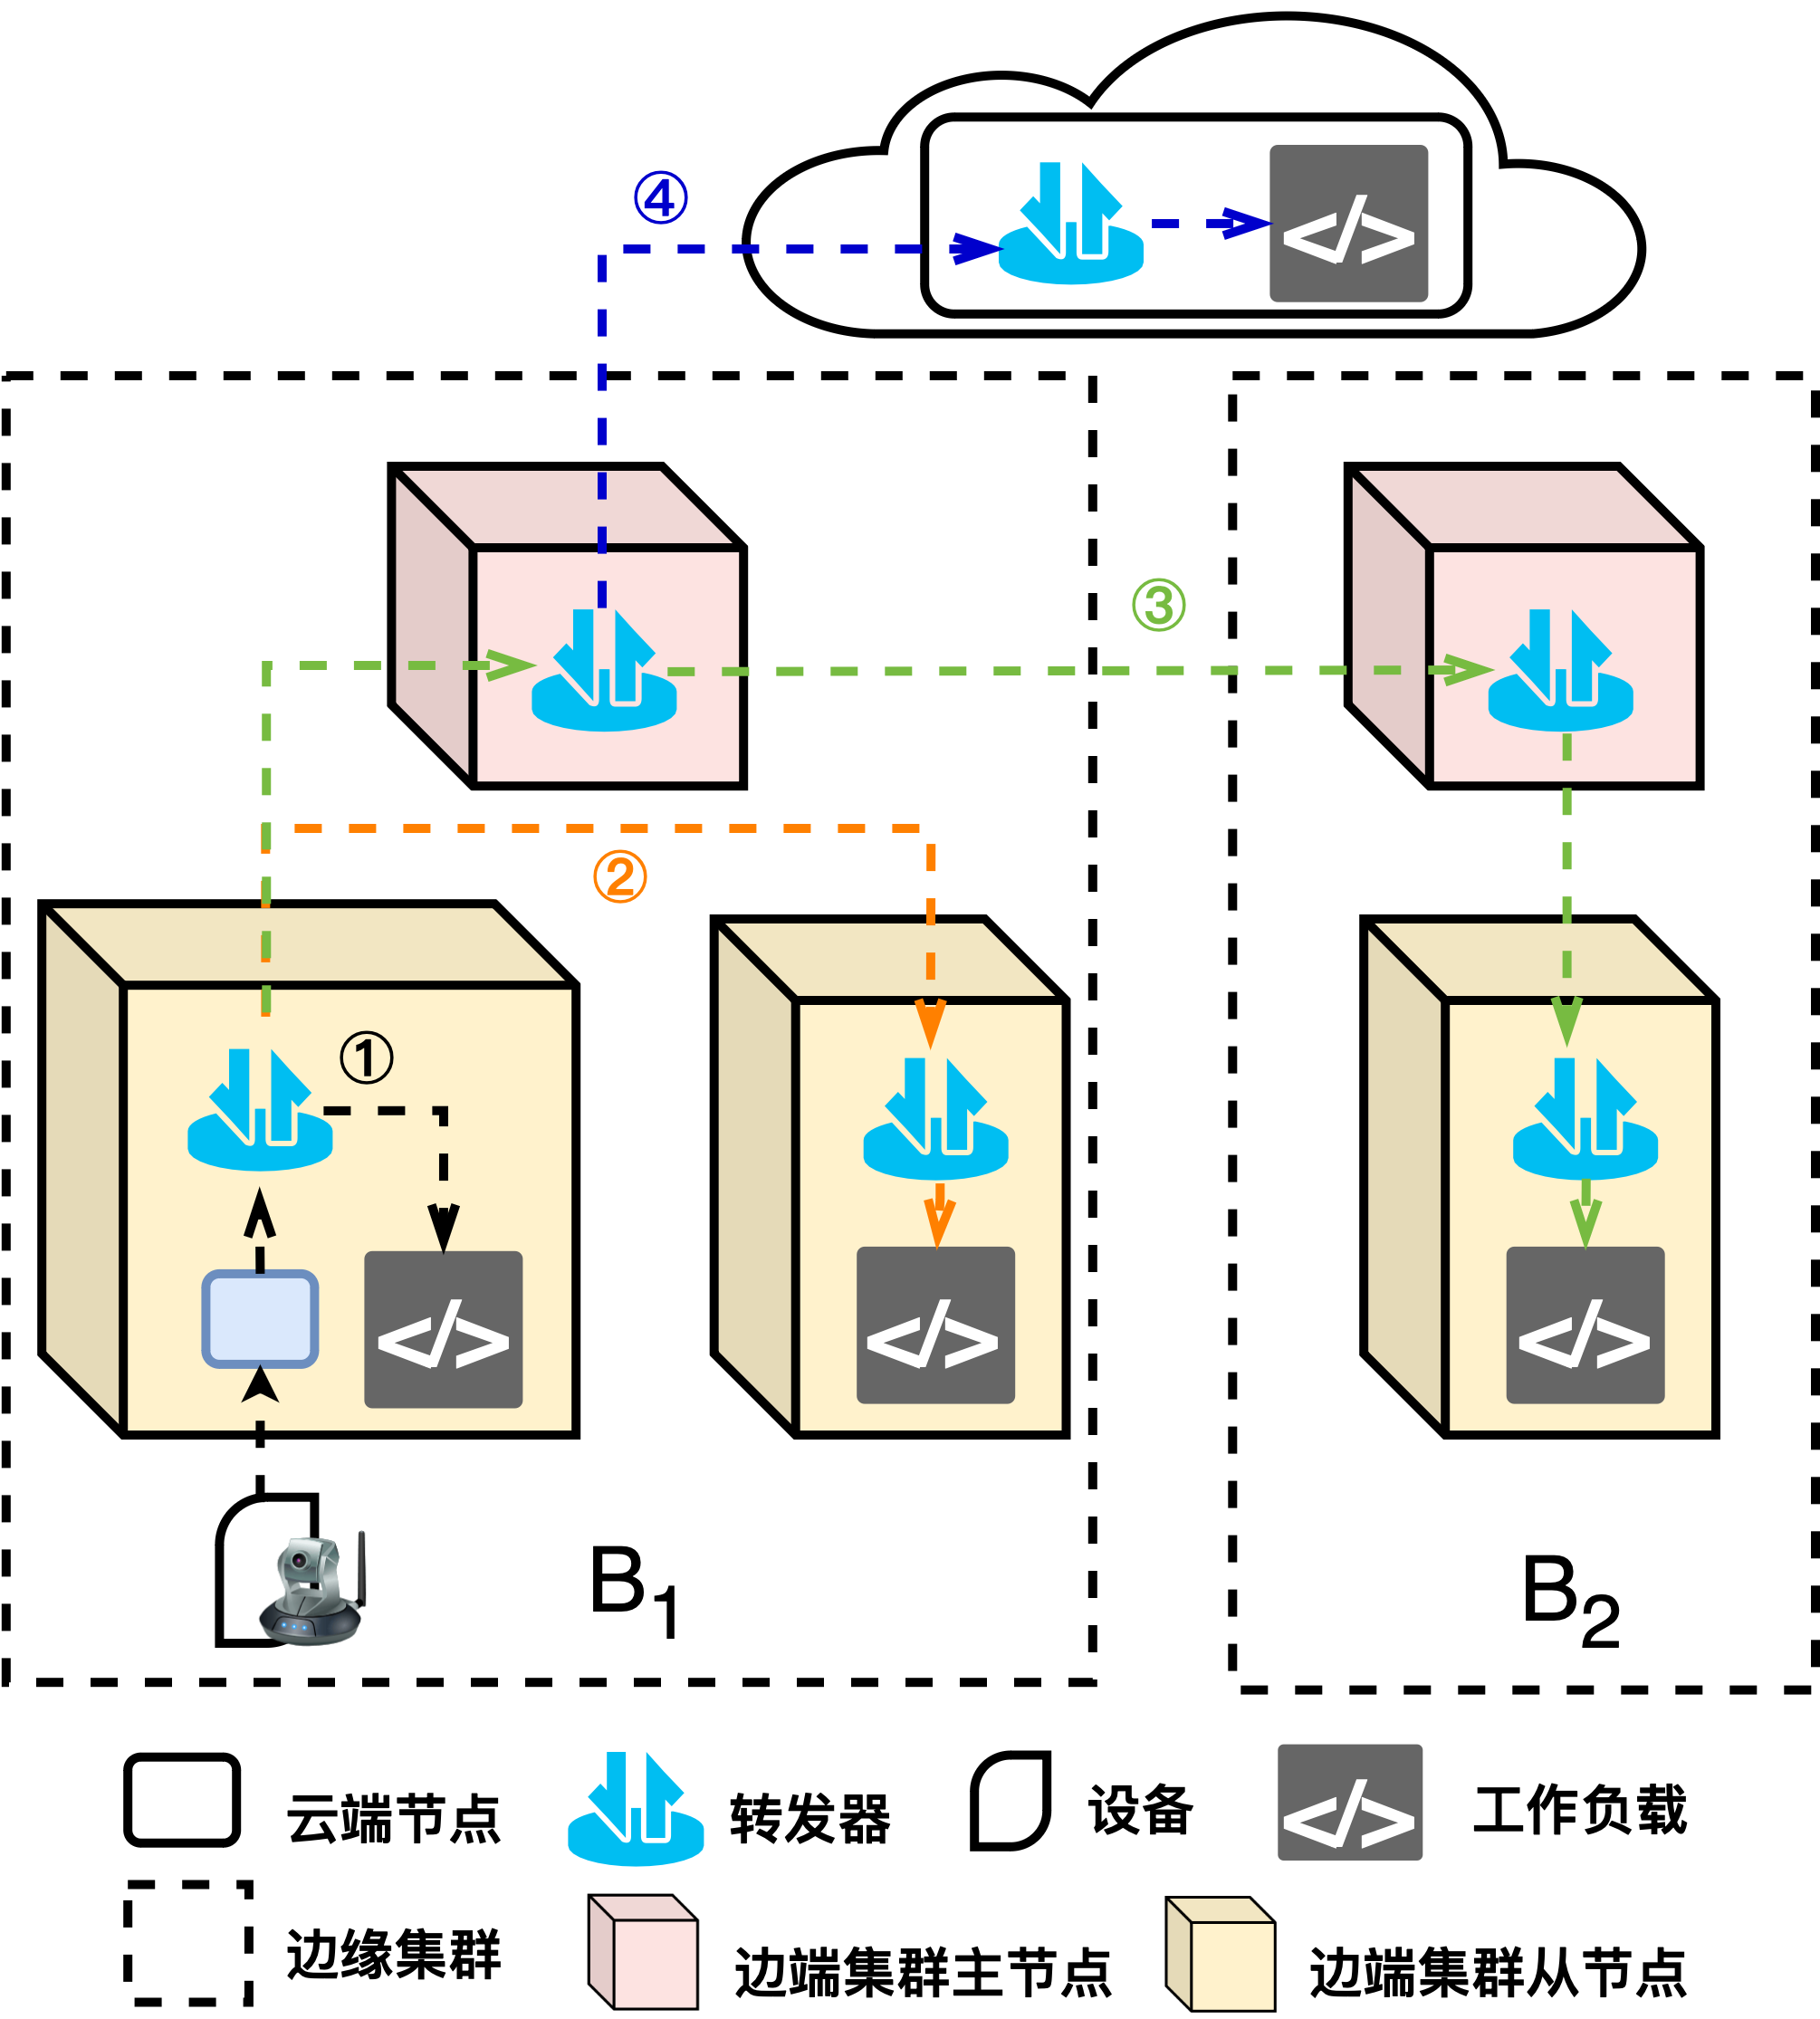
\includegraphics[width=0.6\linewidth]{pics/3-7数据流分流.png}
  \caption{数据流分流场景及其传输模式}
  \label{fig:3-7splitflow}
\end{figure}

对于边缘集群内部的节点间传输,数据在集群$B_k$内从节点$e_{kj}$到$e_{kj'}$的传输过程主要受限于网络物理特性。此时总时延由信号传播时延与数据包传输时延线性叠加构成:

\begin{equation}
    \Theta_{\text{tran}}(e_{kj}, e_{kj'}, G) = \underbrace{\psi_{jj'}^{(k)}}_{\mathclap{\text{传播时延}}} + \underbrace{\frac{G}{\gamma_{jj'}^{(k)}}}_{\mathclap{\text{传输时延}}}
\end{equation}

其中,$\psi_{jj'}^{(k)}$ 表示节点 $e_{kj}$ 和 $e_{kj'}$ 之间的传播时延,$\gamma_{jj'}^{(k)}$ 表示链路带宽。

对于跨集群的数据传输,由边缘节点$e_{kj}$(属于$B_k$)与$e_{lm}$(属于$B_l$)分属不同管理域,数据包需要经过双方主节点的协同路由。该场景下时延模型呈现典型的多跳特征:

\begin{equation}
    \Theta_{\text{tran}}(e_{kj}, e_{lm}, G) = \Theta_{\text{tran}}(e_{kj}, L_k, G) + \underbrace{\psi_{kl}^{\mathrm{ee}} + \frac{G}{\gamma_{kl}^{\mathrm{ee}}}}_{\mathclap{\text{集群间链路开销}}} 
    + \Theta_{\text{tran}}(L_l, e_{lm}, G) 
\end{equation}

其中,$\psi_{kl}^{\mathrm{ee}}$ 和 $\gamma_{kl}^{\mathrm{ee}}$ 分别表示边缘集群间链路的传播时延和带宽。

当数据需要跨越云边边界时,传输路径必须经过边缘集群的主节点$L_k$进行协议转换与路由调度。从边缘节点$e_{kj}$到云端节点$c_q$的端到端时延包含本地转发和云边通道两个阶段:

\begin{equation}
    \Theta_{\text{tran}}(e_{kj}, c_q, G) = \Theta_{\text{tran}}(e_{kj}, L_k, G) + \underbrace{\psi_{kq}^{\mathrm{ce}} + \frac{G}{\gamma_{kq}^{\mathrm{ce}}}}_{\mathclap{\text{云边链路开销}}}
\end{equation}

其中,$\psi_{kq}^{\mathrm{ce}}$ 和 $\gamma_{kq}^{\mathrm{ce}}$ 分别表示云边链路的传播时延和带宽。

\subsubsection{层次化运行时状态}

在动态调度过程中,系统的运行时状态可分解为计算资源状态与数据流转状态两个正交维度。基于定义3.7的计算队列与定义3.11的数据流转图,本文构建运行时状态的形式化模型:

\paragraph{定义3.13 (层次化运行时状态)} 层次化运行时状态$\Upsilon_{t_\omega}^κ$在时间窗$t_\omega$内可表示为一个 2 元组:
\[
\Upsilon_{t_\omega}^κ = (\mathcal{Q}_{t_\omega}^κ, \mathcal{G}_{t_\omega}^κ)
\]
其中:
\begin{itemize}
    \item $\mathcal{Q}_{t_\omega}^κ = \{\mathcal{Q}_s^j(t_\omega)\}_{s \in \mathcal{L}, j \in \mathcal{V}_G^κ}$表示 $\mathcal{V}_G^κ$ 表示上下文相关的队列状态,其作用域由$\mathcal{V}_G^κ$的粒度决定:
        \[
        \mathcal{Q}_{t_\omega}^κ = 
        \begin{cases}
            \{\mathcal{Q}_s^j\}_{s \in \mathcal{L}}, & |\mathcal{V}_G^κ|=1 \ (\exists v_j \in \mathcal{V}) \\
            \bigcup_{e \in \mathcal{B}_k} \{\mathcal{Q}_s^e\}_{s \in \mathcal{L}}, & \mathcal{V}_G^κ = \mathcal{B}_k \ (B_k \in \mathcal{B}) \\
            \{\mathcal{Q}_s^j\}_{s \in \mathcal{L}, j \in \mathcal{V}}, & \mathcal{V}_G^κ = \mathcal{V}
        \end{cases}
        \]
    \item $\mathcal{G}_{t_\omega}^κ = (\mathcal{V}_G^κ, \mathcal{E}_G(t_\omega))$表示动态数据流转图,具体定义详见定义3.12。
\end{itemize}

基于层次化运行时状态$\Upsilon_{t_\omega}^κ$的形式化建模,三级协同调度架构中的各层级调度器可依据其决策域粒度,动态获取适配的系统状态视图。这种层次化状态感知机制使得各层级调度器既能聚焦其决策域内的核心优化目标,又能通过状态参数传递实现跨层协同,形成局部响应与全局优化的动态耦合。

\section{云边协同AI推理分层调度}

\subsection{本地调度}

\subsubsection{本地调度策略}

在节点级调度层面,本地调度器$S_L$的核心目标在于通过动态资源分配策略,优先保障与计算节点$v_j$直连的终端设备$\mathcal{D}_j \subseteq \mathcal{D}$的数据处理需求。如图\ref{fig:3-8localdevice}所示,在时间窗$t_\omega$内,计算节点$v_j$部署的AI负载实例$\ell_s \in \mathcal{L}$在满足本地设备的数据处理请求后,剩余资源方可用于处理外部转发任务。

\begin{figure}[h]
  \centering
  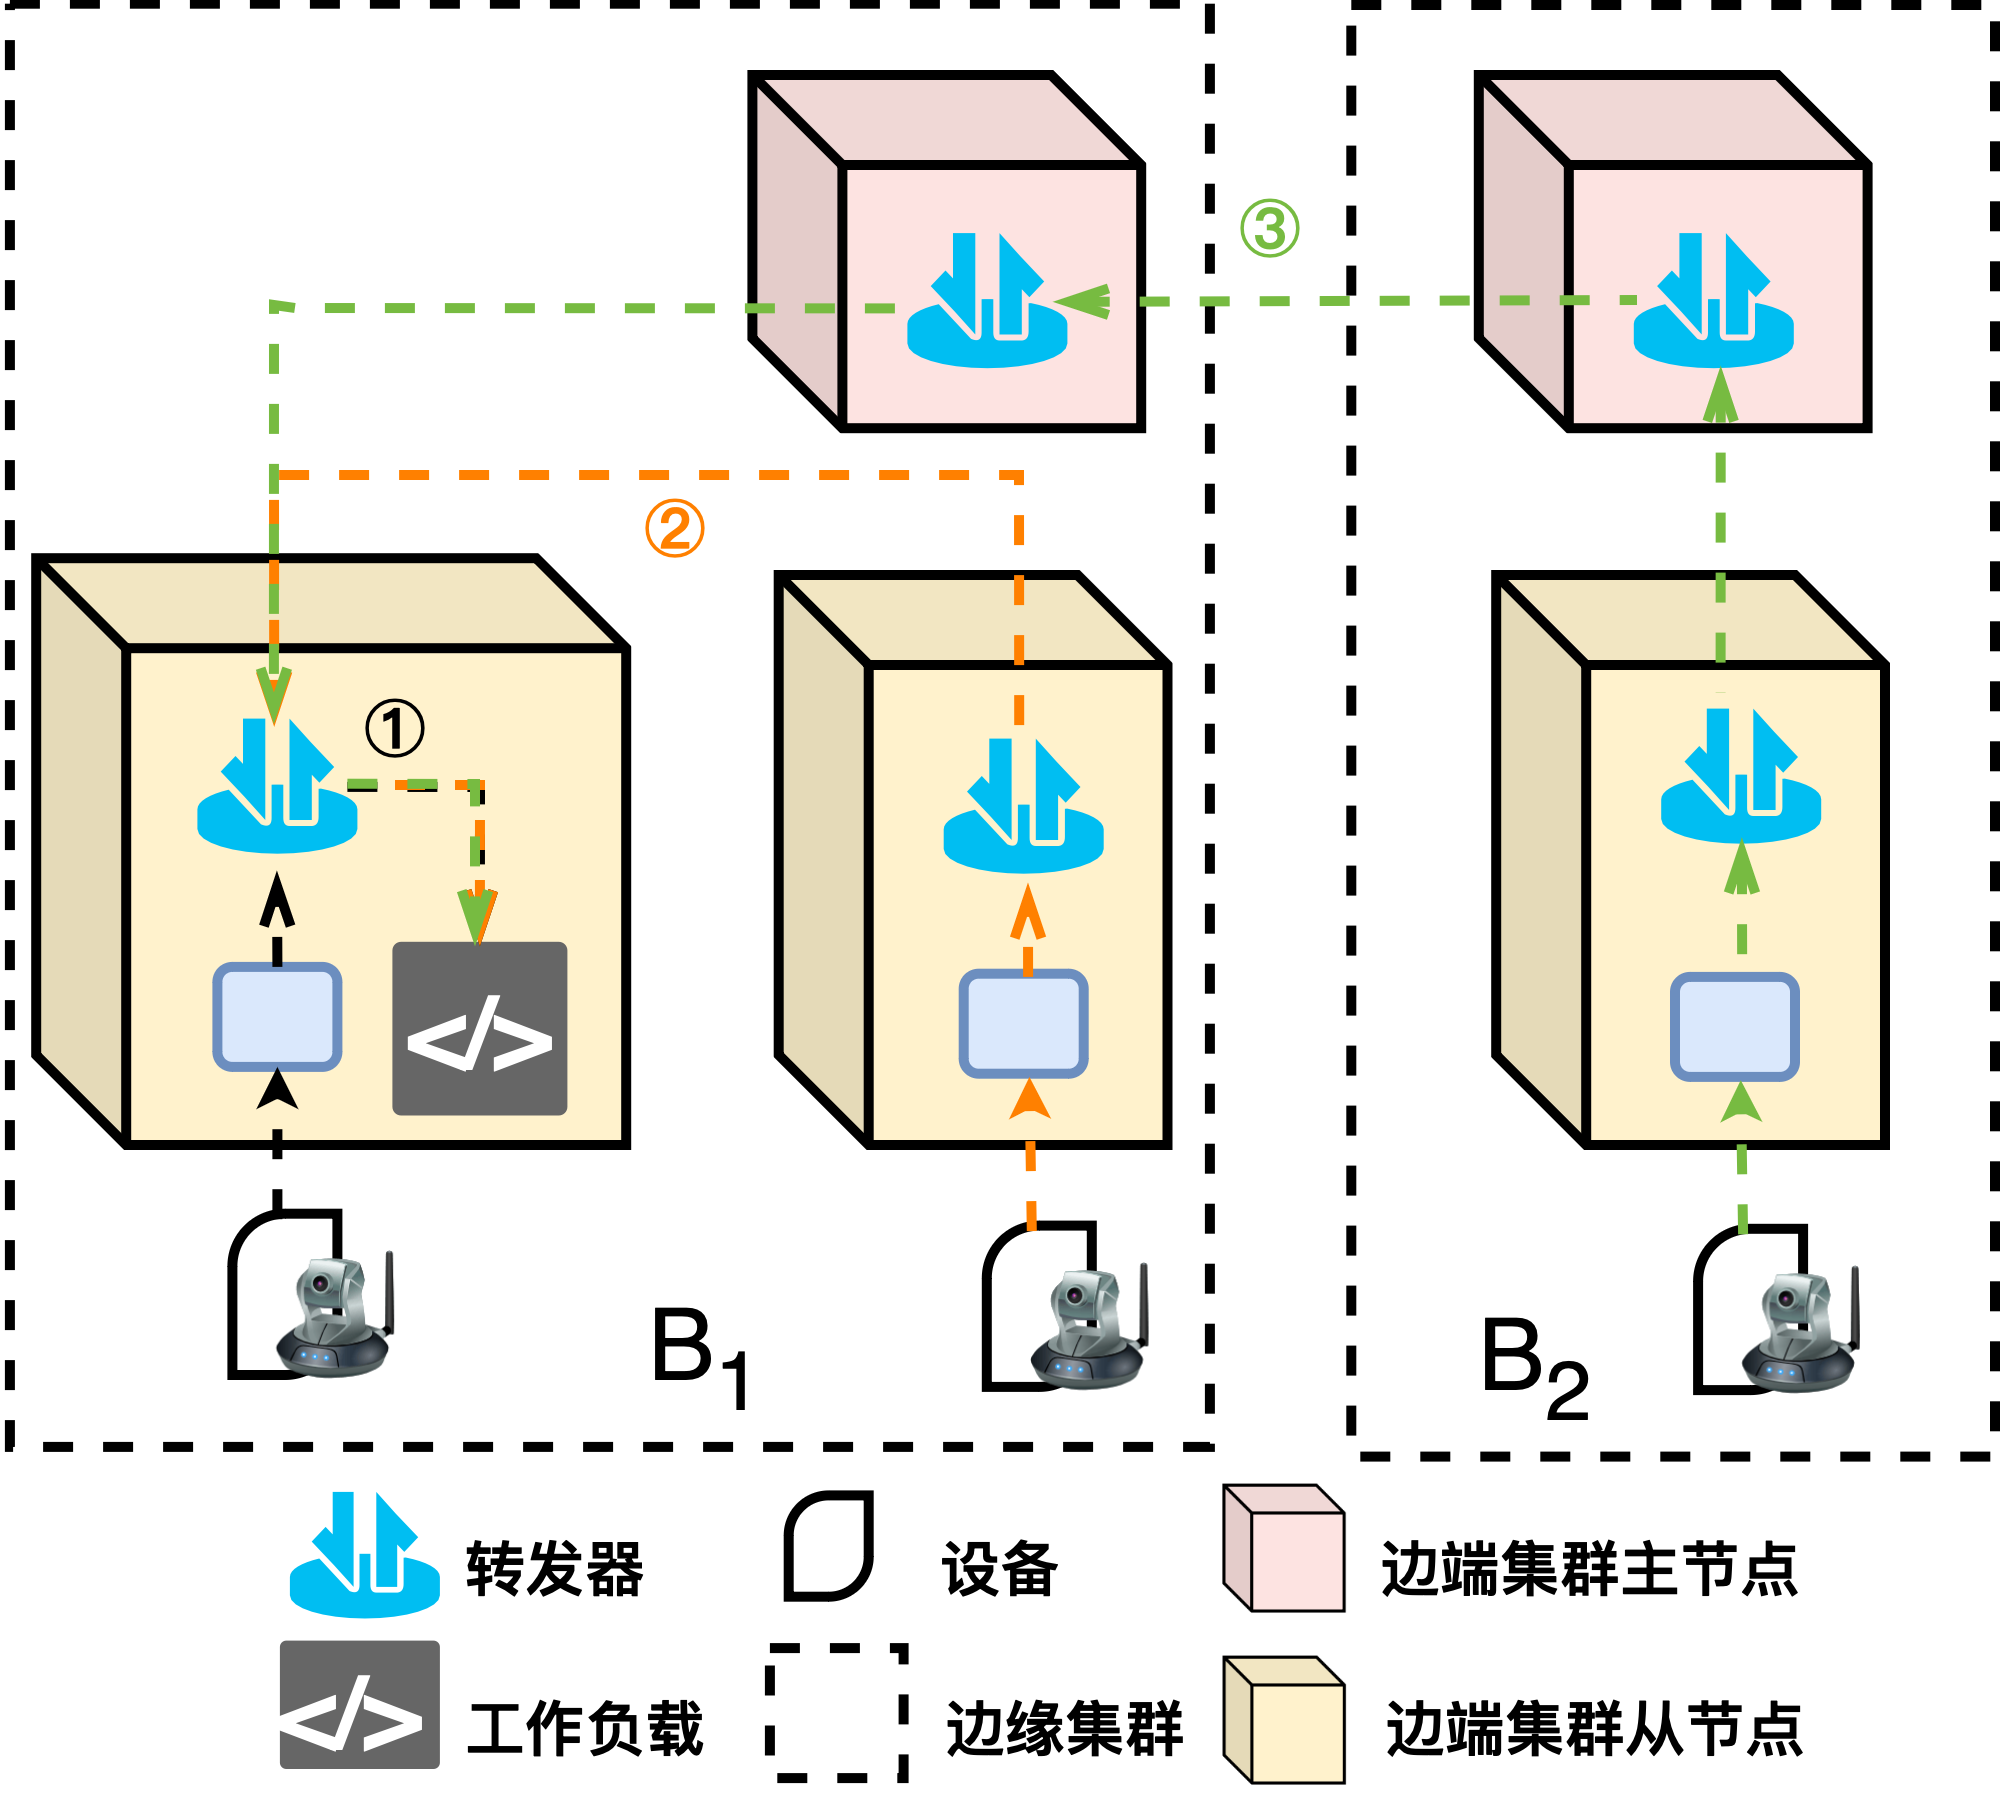
\includegraphics[width=0.6\linewidth]{pics/3-8本地负载处理.png}
  \caption{计算节点本地与外部任务资源调度示意图}
  \label{fig:3-8localdevice}
\end{figure}

当设备$d_i \in \mathcal{D}_j$的瞬时采集频率 $g_i(t)$ 突然增加时,本地节点可能因计算队列容量不足而难以承载所有数据流,本地调度器需通过动态调整分流变量 $\mathcal{Z}_i^{t_\omega}$ ,确保本地设备产生的数据流在计算队列$\mathcal{Q}_s^j(t_\omega)$ 的容量约束下获得优先级保障,从而避免因外部转发任务抢占资源而导致本地服务质量劣化。若本地资源不足,需优先处理单次数据采集量$\varsigma_{i\beta}$最大的设备数据,以最小化跨节点传输开销。其中,决策变量为分流比例$z_{ij}^{t_\omega} \in [0,1]$,表示设备$d_i$的数据流分配至节点$v_j$的比例;优化目标要保证本地服务质量,同时最小化跨节点协作流量,具体如下:

\begin{itemize}
    \item \textbf{本地设备数据流的处理量最大化}:本地节点应优先处理直连设备的流式数据,优化目标可形式化为:
    \[
    \mathop{\text{maximize}} \sum_{d_i \in \mathcal{D}_{j}} z_{ij}^{t_\omega} \cdot g_i^{t_\omega},
    \]
    \item \textbf{跨节点协作流量最小化}:通过最小化跨节点协作处理的数据流量,减少网络传输开销和系统资源消耗,优化目标可形式化为
    \[
    \mathop{\text{minimize}} \sum_{d_i \in \mathcal{D}_j} (1 - z_{ij}^{t_\omega}) \cdot g_i^{t_\omega} \cdot \varsigma_{i\beta}
    \]
\end{itemize}
为了确保上述优化目标的实现,本地调度策略需满足以下约束条件:

\begin{itemize}
    \item \textbf{计算队列容量约束}:本地与外部数据流的总分配量不得超过节点$v_j$的计算能力极限。具体而言,分配至节点的数据采集量应满足:
    \[
    \sum_{d_i \in \mathcal{D}} z_{ij}^{t_\omega} \cdot g_i^{t_\omega} \leq \Lambda_s^j(t_\omega) \quad \forall \ell_s \in \mathcal{L}_j,
    \]
    其中$\mathcal{D}$表示本地与外部终端设备的并集。
    
    \item \textbf{分流完整性约束}:每个本地设备的数据流需完整分配至计算节点集合,确保数据流不丢失且合理分布。具体而言,分流变量需满足完整性约束:
    \[
    \sum_{v_l \in \mathcal{V}} z_{il}^{t_\omega} = 1 \quad \forall d_i \in \mathcal{D}_j,
    \]
    其中,$\mathcal{V}$表示所有可用计算节点的集合,分流变量 $z_{ij}^{t_\omega}$ 的取值范围需满足 $z_{ij}^{t_\omega} \in [0,1]$。

    \item \textbf{资源适配性约束}:AI 负载实例 $\ell_s$ 需要与节点 $v_j$ 的资源供给和硬件架构相匹配,以确保负载实例能够顺利部署并高效运行。具体而言,需满足以下条件:
    \[
    \rho_j \geq \mathcal{R}_s \quad \text{且} \quad \alpha_j \in \mathcal{A}_s,
    \]
    其中$\rho_j$ 和 $\mathcal{R}_s$ 分别表示节点 $v_j$ 的资源供给向量和负载实例 $\ell_s$ 的资源需求向量;$\alpha_j$ 和 $\mathcal{A}_s$ 分别表示节点 $v_j$ 的硬件架构和负载实例 $\ell_s$ 的硬件架构需求。
\end{itemize}

综上所述,本地调度策略的优化问题可形式化为以下多目标模型:

\[
\begin{aligned}
\mathop{\text{maximize}}\quad & \sum_{d_i \in \mathcal{D}_j} z_{ij}^{t_\omega} \cdot g_i^{t_\omega} \\
\mathop{\text{minimize}}\quad & \sum_{d_i \in \mathcal{D}_j} (1 - z_{ij}^{t_\omega}) \cdot g_i^{t_\omega} \cdot \varsigma_{i\beta} \\
\text{s.t.}\quad 
& \sum_{d_i \in \mathcal{D}} z_{ij}^{t_\omega} \cdot g_i^{t_\omega} \leq \Lambda_s^j(t_\omega) \\
& \sum_{v_l \in \mathcal{V}} z_{il}^{t_\omega} = 1,\ \forall d_i \in \mathcal{D}_j ,\ 0 \leq z_{ij}^{t_\omega} \leq 1\\
& \rho_j \geq \mathcal{R}_s,\ \alpha_j \in \mathcal{A}_s
\end{aligned}
\label{eq:local_scheduling}
\]


\subsubsection{本地调度优化算法}

基于上述优化策略,本文提出基于贪心策略的本地调度优化算法。该算法通过构建优先级队列,以本地设备单次数据采集量$\varsigma_{i\beta}$为依据,确保本地设备的数据流能够优先获得调度资源,同时有效减少跨节点传输的开销。在此基础上,算法还引入了弹性容量分配机制,在严格满足计算队列容量约束的前提下,动态调整数据分流比例。这一机制不仅能够保障本地服务质量,还能最大化系统吞吐量,从而在资源利用与性能需求之间实现平衡。具体算法流程如算法\ref{alg:local_scheduling}所示。

\begin{algorithm}[ht]
\caption{本地调度算法}
\label{alg:local_scheduling}
\begin{algorithmic}[1]
\REQUIRE  
  直连设备集合$\mathcal{D}_j$,  节点$v_j$在$t_\omega$时间窗的计算容量$C^{t_\omega}_j$, 设备流式数据特征元组$\{(g_i^{t_\omega}, \varsigma_{i\beta})\}_{d_i \in \mathcal{D}_j}$
\ENSURE  
  设备到节点的分流比例集合$\{z_{ij}^{t_\omega}\}$

\STATE 初始化分流比例 $z_{ij}^{t_\omega} \leftarrow 0,\ \forall d_i \in \mathcal{D}_j$  
\STATE 剩余可用容量 $R \leftarrow C_j^{t_\omega}$  

\STATE 生成设备优先级队列 $\mathcal{P} \leftarrow \textsc{Sort}(\mathcal{D}_j, \varsigma_{i\beta} \downarrow)$  
  \COMMENT{按单次数据量$\varsigma_{i\beta}$降序排序}

\WHILE{$\mathcal{P} \neq \emptyset$ \AND $R > 0$}
  \STATE 取出队首设备 $d_i \leftarrow \mathcal{P}.\textsc{Dequeue}()$
  \STATE 计算资源需求 $u_i \leftarrow g_i^{t_\omega} \times \varsigma_{i\beta}$ 
  
  \IF{$u_i \leq R$}
    \STATE $z_{ij}^{t_\omega} \leftarrow 1.0$ \COMMENT{全量本地化处理}
    \STATE $R \leftarrow R - u_i$ \COMMENT{更新剩余容量}
  \ELSE
    \STATE $z_{ij}^{t_\omega} \leftarrow R / u_i$ \COMMENT{按比例分配剩余容量}
    \STATE $R \leftarrow 0$ \COMMENT{触发资源耗尽状态}
  \ENDIF
\ENDWHILE
\RETURN $\{z_{ij}^{t_\omega}\}_{d_i \in \mathcal{D}_j}$
\end{algorithmic}
\end{algorithm}

算法\ref{alg:local_scheduling}的总体时间复杂度为$O(|\mathcal{D}_j| \log |\mathcal{D}_j|)$,其中通过排序函数 $\textsc{Sort}$ 构建设备优先级队列 $\mathcal{P}$的时间复杂度为 $O(|\mathcal{D}_j| \log |\mathcal{D}_j|)$,主循环逐一处理优先级队列中的设备的时间复杂度为 $O(|\mathcal{D}_j|)$。


\subsection{边缘集群调度}

\subsubsection{边缘集群调度策略}

在实际运行过程中,本地节点$v_j$可能因多重约束无法有效处理直连设备$d_i \in \mathcal{D}_j$的数据请求。例如,当设备$d_i$的瞬时采集频率 $g_i(t)$ 突然增加时,本地节点的计算队列容量可能无法承载骤增的数据流;若本地节点的硬件架构与AI负载实例不兼容,或资源供给不足,则无法部署所需的计算任务;当节点处于节能模式或能源受限时,可能仅保留基础数据转发功能,而无法执行完整的AI推理任务。如图\ref{fig:3-9edgecluster}所示,当上述情况发生时,本地节点$v_j$首先在本地调度阶段确定分流比例$z_{ij}^{t_\omega}$,将占比  $z_{ij}^{t_\omega}$ 的数据流进行本地处理,剩余未处理数据流$g_{i,\text{res}}^{t_\omega} = g_i^{t_\omega} \cdot (1 - z_{ij}^{t_\omega})$将进入集群级再分配流程。

\begin{figure}[h]
  \centering
  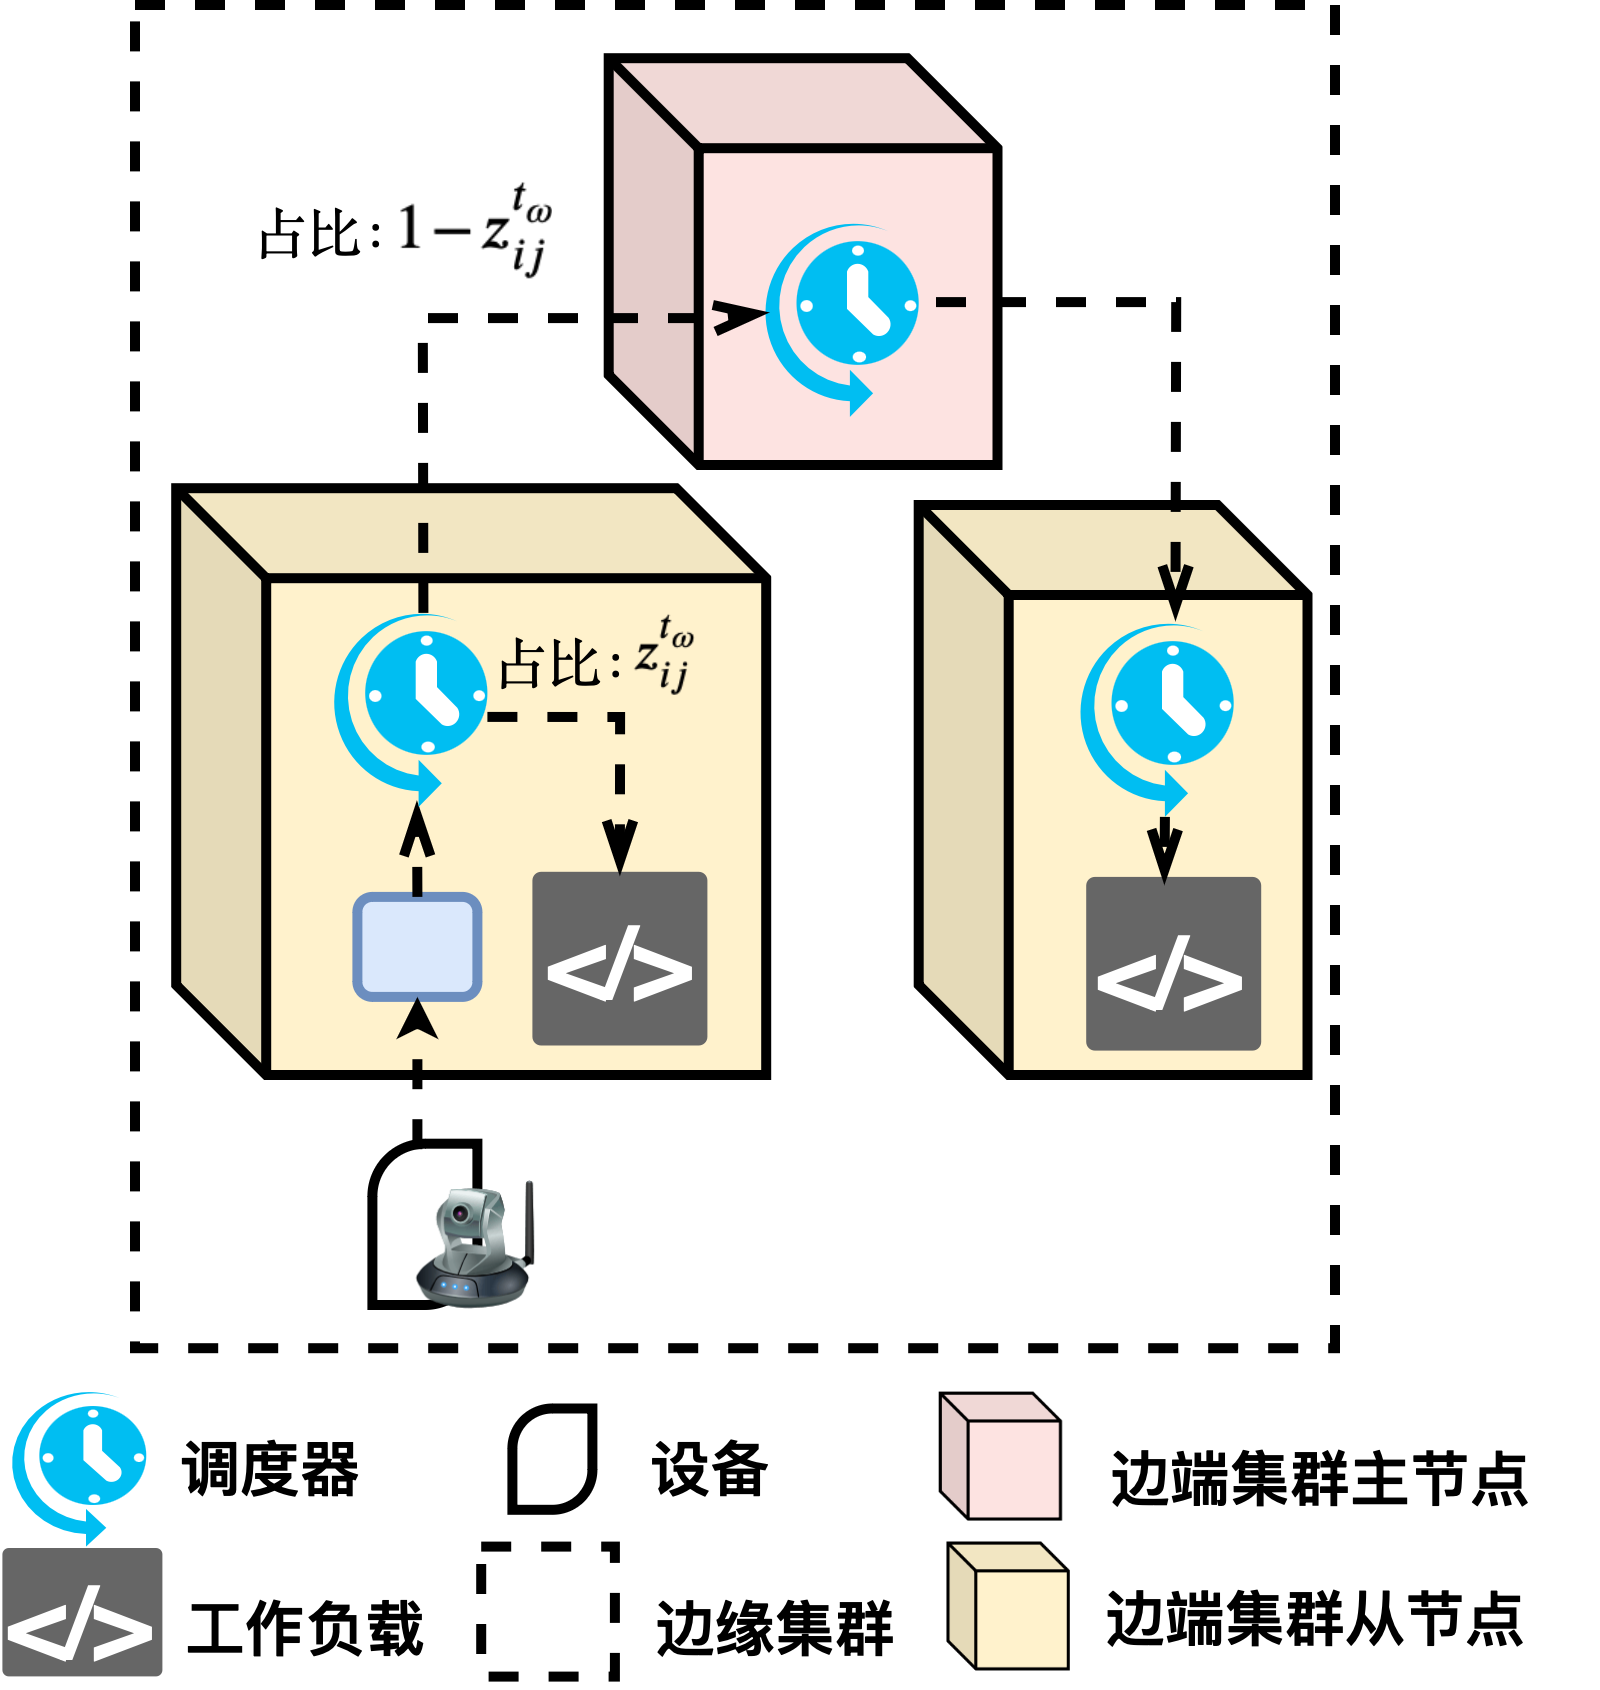
\includegraphics[width=0.5\linewidth]{pics/3-9集群内部调度.png}
  \caption{本地节点设备数据流分流过程}
  \label{fig:3-9edgecluster}
\end{figure}

在边缘集群内部调度层面,边缘集群调度器$S_B$需在集群$B_k$的节点集合$\mathcal{E}_k$中动态分配数据流,同时优化跨节点协作产生的传输开销。其中,决策变量为剩余分流比例$\{z_{ikj}^{t_\omega}\}_{e_{kj} \in \mathcal{E}_k \setminus v_j}$,其取值范围为$[0,1]$,表示设备$d_i$的剩余数据分配至集群内节点$e_{kj}$的比例;优化目标要兼顾时延敏感性,保证集群内部的服务质量,并减少跨域流量,具体如下:

\begin{itemize}
    \item \textbf{端到端时延最小化}:总时延由推理时延与传输时延两部分构成。对于设备 $d_i$ 的数据流分配至节点 $e_{kj}$的情形,总时延可分解为:
    \[
    \Theta_{\text{total}} = \underbrace{\Theta_{\text{inf}}(\ell_s, e_{kj})}_{\text{推理时延}} + \underbrace{\Theta_{\text{tran}}(e_{kj'}, e_{kj}, G_{ik}^{t_\omega})}_{\mathclap{\text{集群内传输时延}}}
    \]
    其中,$e_{kj'}$ 为设备的原始本地节点,$G_{ik}^{t_\omega} = g_{i,\text{res}}^{t_\omega} \cdot z_{ikj}^{t_\omega} \cdot \varsigma_\beta$ 表示设备 $d_i$ 分配至节点 $e_{kj}$ 的数据流量。优化目标可形式化为:
    \[
    \mathop{\text{minimize}} \sum_{d_i \in \mathcal{D}} \sum_{e_{kj} \in \mathcal{E}_k \setminus v_j} z_{ikj}^{t_\omega} \cdot \Theta_{\text{total}}
    \]
    即最小化所有设备数据流在集群内部节点间的端到端时延。
    \item \textbf{集群内部设备数据流处理量最大化}:边缘集群应优先处理其集群内部直连设备的数据流,优化目标可形式化为:
    \[
   \mathop{\text{maximize}} \sum_{d_i \in \mathcal{D}_k} \sum_{e_{kj} \in \mathcal{E}_k \setminus v_j} z_{ikj}^{t_\omega},
   \]
   其中 $\mathcal{D}_k$ 表示归属集群 $B_k$ 的终端设备集合。
   \item \textbf{跨域协作流量最小化}:最小化跨域协作处理的数据流量,优化目标可形式化为
    \[
    \mathop{\text{minimize}} \sum_{d_i \in \mathcal{D}_k} \left(1 - \sum_{e_{kj} \in \mathcal{E}_k \setminus v_j} z_{ikj}^{t_\omega}\right) \cdot g_{i,\text{res}} \cdot \varsigma_\beta
    \]
\end{itemize}
为了确保上述优化目标的实现,集群内部调度策略需满足以下约束条件:

\begin{itemize}
    \item \textbf{边缘集群计算队列容量约束}:  
    边缘集群内所有节点的计算队列总容量不得超过其最大吞吐量限制。具体而言,分配至每个节点的数据采集量应满足:
    \[
    \sum_{d_i \in \mathcal{D}} z_{ikj}^{t_\omega} \cdot g_i^{t_\omega} \leq \Lambda_s^{kj}(t_\omega) \quad \forall e_{kj} \in \mathcal{E}_k,
    \]
    其中,$\Lambda_s^{kj}(t_\omega)$ 表示节点 $e_{kj}$ 在时间窗 $t_\omega$ 内对负载实例 $\ell_s$ 的最大吞吐量,$\mathcal{D}$表示全部的终端设备设备。
    
    \item \textbf{边缘集群设备数据流完整性约束}:边缘集群中每个设备的数据流需完整分配至计算节点集合,确保每个设备的数据流被完整分配且不丢失。具体而言,分流变量需满足完整性约束:
    \[
    \sum_{v_l \in \mathcal{V}} z_{l}^{t_\omega} = 1 \quad \forall d_i \in \mathcal{D}_k \quad z_{l}^{t_\omega} \in [0, 1], 
    \]
    其中,$\mathcal{V}$表示所有可用计算节点的集合,$\mathcal{D}_k$ 表示归属集群 $B_k$ 的终端设备集合。
    
    \item \textbf{边缘集群设备资源适配性约束}:AI 负载实例 $\ell_s$ 需要与目标节点 $e_{kj}$ 的资源供给和硬件架构相匹配。具体而言,需满足以下条件:
    \[
    \rho_{kj} \geq \mathcal{R}_s \quad \text{且} \quad \alpha_{kj} \in \mathcal{A}_s \quad \forall e_{kj} \in \mathcal{E}_k ,
    \]
    其中,$\rho_{kj}$ 和 $\mathcal{R}_s$ 分别表示节点 $e_{kj}$ 的资源供给向量和负载实例 $\ell_s$ 的资源需求向量;$\alpha_{kj}$ 和 $\mathcal{A}_s$ 分别表示节点 $e_{kj}$ 的硬件架构和负载实例 $\ell_s$ 的硬件架构需求。
\end{itemize}

综上所述,边缘集群内部调度策略的优化问题可形式化为以下多目标模型:

\[
\begin{aligned}
\mathop{\text{minimize}}\quad & \sum_{d_i \in \mathcal{D}} \sum_{e_{kj} \in \mathcal{E}_k} z_{ikj}^{t_\omega} \cdot \Theta_{\text{total}} \\
\mathop{\text{maximize}}\quad & \sum_{d_i \in \mathcal{D}_{B_k}} \sum_{e_{kj} \in \mathcal{E}_k} z_{ikj}^{t_\omega} \cdot g_i^{t_\omega} \\
\text{s.t.}\quad 
& \sum_{d_i \in \mathcal{D}_{B_k}} z_{ikj}^{t_\omega} \cdot g_i^{t_\omega} \leq \Lambda_s^{kj}(t_\omega), \quad \forall e_{kj} \in \mathcal{E}_k \\
& \sum_{v_{l} \in \mathcal{V}} z_{il}^{t_\omega} = 1, \quad z_{il}^{t_\omega} \in [0,1], \quad \forall d_i \in \mathcal{D}_{B_k} \\
& \rho_{kj} \geq \mathcal{R}_s, \quad \alpha_{kj} \in \mathcal{A}_s, \quad \forall e_{kj} \in \mathcal{E}_k 
\end{aligned}
\label{eq:cluster_scheduling}
\]

\subsubsection{边缘集群调度优化算法}

基于上述优化策略,本文提出了一种结合贪心策略与多维度优先级队列的边缘集群调度优化算法。该算法首先根据设备单次数据采集量$\varsigma_{i\beta}$对流式数据进行优先级排序,构建初始优先级队列,确保本集群内的设备数据能够优先获得调度资源,从而有效减少跨集群和云边传输的开销。在此基础上,针对每条流式数据,算法筛选出集群中具有剩余计算队列容量的候选节点,并进一步依据端到端时延建立时延优先队列。通过引入时延敏感度感知机制,算法有效降低了集群内部调度的总时延,同时满足任务的时延约束要求。此外,算法采用动态分配策略,在候选节点间按剩余容量比例分配数据流,既避免了单一节点过载问题,又最大化了集群内部计算资源的利用率。通过这一机制,算法在保证服务质量的同时实现了高效的资源调度与任务分配,具体流程详见算法\ref{alg:cluster_scheduling}。

\begin{algorithm}[ht]
\caption{边缘集群调度算法}
\label{alg:cluster_scheduling}
\begin{algorithmic}[1]
\REQUIRE  
  集群$B_k$待调度数据流集合$\mathcal{F}_k$, 集群节点剩余容量$\{C^{t_\omega}_m\}_{e_{km} \in \mathcal{E}_k}$, 时延与带宽参数$\{\Theta_{\text{total}}(e_{km})\}$, 单次采集量$\varsigma_\beta$
\ENSURE  
  数据流到集群节点的分流比例集合$\{z_{ikm}^{t_\omega}\}$

\STATE 初始化分流比例 $z_{ikm}^{t_\omega} \leftarrow 0,\ \forall f_i \in \mathcal{F}_k, e_{km} \in \mathcal{E}_k$  
\STATE 生成数据流队列 $\mathcal{Q} \leftarrow \textsc{Sort}(\mathcal{F}_k, \varsigma_\beta \downarrow)$  
  \COMMENT{按单次数据量$\varsigma_{i\beta}$降序排序}

\FOR{每个数据流 $f_i \in \mathcal{Q}$} 
  \STATE 获取候选节点集 $\mathcal{N}_i \leftarrow \textsc{FilterNodes}()$  
    \COMMENT{筛选兼容且有剩余容量的节点}
  \STATE 生成时延优先级队列 $\mathcal{M}_i \leftarrow \textsc{Sort}(\mathcal{N}_i, \Theta_{\text{total}} \uparrow)$  
    \COMMENT{按端到端时延升序排序}
  \STATE 剩余待分配量 $r_i \leftarrow g_{i,\text{res}}^{t_\omega}$

  \WHILE{$r_i > 0$ \AND $\mathcal{M}_i \neq \emptyset$}
    \STATE 取出队首节点 $e_{km} \leftarrow \mathcal{M}_i.\textsc{Dequeue}()$
    \STATE 可用容量 $a_m \leftarrow C^{t_\omega}_m - \sum_{f_j \in \mathcal{F}_k} z_{jkm}^{t_\omega} \cdot g_{j,\text{res}}^{t_\omega}$
    
    \IF{$a_m \geq r_i$}
      \STATE $z_{ikm}^{t_\omega} \leftarrow r_i / g_{i,\text{res}}^{t_\omega}$  
        \COMMENT{全量分配给当前节点}
      \STATE 更新节点容量占用 $C^{t_\omega}_m \leftarrow C^{t_\omega}_m - r_i$
      \STATE $r_i \leftarrow 0$
    \ELSE
      \STATE $z_{ikm}^{t_\omega} \leftarrow a_m / g_{i,\text{res}}^{t_\omega}$  
        \COMMENT{按剩余容量比例分配}
      \STATE 更新节点容量占用 $C^{t_\omega}_m \leftarrow 0$
      \STATE $r_i \leftarrow r_i - a_m$
    \ENDIF
  \ENDWHILE
\ENDFOR
\RETURN $\{z_{ikm}^{t_\omega}\}$
\end{algorithmic}
\end{algorithm}

算法\ref{alg:cluster_scheduling}的总体时间复杂度为$O(|\mathcal{F}_k| \log |\mathcal{F}_k| + |\mathcal{F}_k| \cdot |\mathcal{E}_k| \log |\mathcal{E}_k|)$,其中生成数据流优先级队列的时间复杂度为$O(|\mathcal{F}_k| \log |\mathcal{F}_k|)$,而针对每个数据流的候选节点筛选和时延排序的时间复杂度为$O(|\mathcal{E}_k| \log |\mathcal{E}_k|)$。主循环部分的时间复杂度为$O(|\mathcal{F}_k| \cdot |\mathcal{E}_k|)$,确保了算法在大规模集群环境下的可扩展性。

\subsection{云端全局调度}

\subsubsection{云端全局调度策略}

在全局调度层面,云端全局调度器$S_C$需协调跨边缘集群与云端的资源,处理经过本地与集群调度后仍未完成的剩余数据流。当边缘集群$B_k$的节点集合$\mathcal{E}_k$无法完全处理其中节点$v_j$关联设备的请求时,剩余数据流$g_{i,\text{res}}^{t_\omega} = g_i^{t_\omega} \cdot \left(1 - \sum_{e_{kj} \in \mathcal{E}_k} z_{ikj}^{t_\omega}\right)$将被转发至全局资源池进行再分配。决策变量为全局分流比例$\{z_{ikq}^{t_\omega}\}_{v_q \in \mathcal{V} \setminus \mathcal{E}_k}$,其中$z_{ikq}^{t_\omega} \in [0,1]$表示设备$d_i$的剩余数据分配至节点$v_q$(包括其他边缘集群节点或云端节点)的比例。全局调度策略的优化目标需兼顾时延敏感性与跨域带宽效率:
\begin{itemize}
    \item \textbf{端到端时延最小化}:总时延由推理时延与跨层级传输时延构成。对于设备$d_i$的数据流分配至节点$v_q$的情形,总时延可分解为:
    \[
    \Theta_{\text{total}} = \underbrace{\Theta_{\text{inf}}(\ell_s, v_q)}_{\text{推理时延}} + \underbrace{\Theta_{\text{tran}}(L_k, v_q, G_{ikq}^{t_\omega})}_{\mathclap{\text{跨域传输时延}}}
    \]
    其中$G_{ikq}^{t_\omega} = g_{i,\text{res}}^{t_\omega} \cdot z_{ikq}^{t_\omega} \cdot \varsigma_\beta$为待传输数据量。优化目标可形式化为:
    \[
    \mathop{\text{minimize}} \sum_{d_i \in \mathcal{D}} \sum_{v_q \in \mathcal{V} \setminus \mathcal{E}_k} z_{ikq}^{t_\omega} \cdot \Theta_{\text{total}}
    \]

    \item \textbf{跨域带宽占用最小化}:为降低广域网带宽消耗,需最小化跨边缘集群间及云边链路的带宽占用总量。目标函数可表示为:
    \[
    \mathop{\text{minimize}} \sum_{B_k \in \mathcal{B}} \sum_{v_q \in \mathcal{V} \setminus \mathcal{B}_k} \frac{G_{ikq}^{t_\omega}}{\Gamma_{kq}^{\text{type}}}
    \]
    其中$\Gamma_{kq}^{\text{type}} = \begin{cases}
        \gamma_{kl}^{\mathrm{ee}} & \text{若} v_q \in B_l \ (l \neq k) \\
        \gamma_{kq}^{\mathrm{ce}} & \text{若} v_q \in \mathcal{C}
    \end{cases}$表示对应链路的有效带宽。
\end{itemize}
为了确保上述优化目标的实现,全局调度策略需满足以下约束条件:

\begin{itemize}
    \item \textbf{全局计算队列容量约束}:所有计算节点的分配负载不得超过其最大吞吐量:
    \[
    \sum_{d_i \in \mathcal{D}} z_{ikq}^{t_\omega} \cdot g_i^{t_\omega} \leq \Lambda_s^q(t_\omega), \quad \forall v_q \in \mathcal{V}
    \]
    其中,$\Lambda_s^{q}(t_\omega)$ 表示节点 $v_{q}$ 在时间窗 $t_\omega$ 内对负载实例 $\ell_s$ 的最大吞吐量,$\mathcal{D}$表示全部的终端设备设备。

    \item \textbf{全局分流完整性约束}:剩余数据流需完整分配至全局计算节点:
    \[
    \sum_{v_q \in \mathcal{V}} z_{ikq}^{t_\omega} = 1, \quad z_{ikq}^{t_\omega} \in [0,1], \quad \forall d_i \in \mathcal{D}
    \]
    其中,$\mathcal{V}$表示所有可用计算节点的集合,$\mathcal{D}$ 表示所有终端设备集合。

    \item \textbf{全局资源适配性约束}:AI 负载实例 $\ell_s$ 需要与目标节点 $v_q$ 的资源供给和硬件架构相匹配。具体而言,需满足以下条件:
    \[
    \rho_q \geq \mathcal{R}_s \quad \text{且} \quad \alpha_q \in \mathcal{A}_s, \quad \forall v_q \in \mathcal{V}
    \]
    其中,$\rho_{q}$ 和 $\mathcal{R}_s$ 分别表示节点 $v_q$ 的资源供给向量和负载实例 $\ell_s$ 的资源需求向量;$\alpha_q$ 和 $\mathcal{A}_s$ 分别表示节点 $v_q$ 的硬件架构和负载实例 $\ell_s$ 的硬件架构需求。


\end{itemize}

综上所述,全局调度策略的优化问题可形式化为以下多目标模型:

\[
\begin{aligned}
\mathop{\text{minimize}}\quad & \sum_{d_i \in \mathcal{D}} \sum_{v_q \in \mathcal{V} \setminus \mathcal{B}_k} z_{ikq}^{t_\omega} \cdot \Theta_{\text{total}} \\
\mathop{\text{minimize}}\quad & \sum_{B_k \in \mathcal{B}} \sum_{v_q \in \mathcal{V} \setminus \mathcal{B}_k} \frac{G_{ikq}^{t_\omega}}{\Gamma_{kq}^{\text{type}}} \\
\text{s.t.}\quad 
& \sum_{d_i \in \mathcal{D}} z_{ikq}^{t_\omega} \cdot g_i^{t_\omega} \leq \Lambda_s^q(t_\omega), \quad \forall v_q \in \mathcal{V} \\
& \sum_{v_q \in \mathcal{V} } z_{ikq}^{t_\omega} = 1, \quad \forall d_i \in \mathcal{D}, \quad z_{ikq}^{t_\omega} \in [0,1] \\
& \rho_q \geq \mathcal{R}_s, \quad \alpha_q \in \mathcal{A}_s, \quad \forall v_q \in \mathcal{V} 
\end{aligned}
\label{eq:global_scheduling}
\]

\subsubsection{云端全局调度优化算法}

基于上述优化策略,本文首先采用线性函数归一化(Min-Max Scaling)方法消除目标函数之间的量纲差异。具体而言,设时延目标的最大值和最小值分别为 $J_1^{\max}$ 和 $J_1^{\min}$,带宽目标的最大值和最小值分别为 $J_2^{\max}$ 和 $J_2^{\min}$,则归一化公式为:
\[
\hat{J}_k = \frac{J_k - J_k^{\min}}{J_k^{\max} - J_k^{\min}},\quad k=1,2
\]
通过归一化处理,可以将多目标优化问题转化为统一的无量纲形式,便于后续求解。理论上,归一化后的优化问题可以通过数学规划工具(如 OR-Tools\cite{google_or_tools})进行精确求解。然而,精确算法的时间复杂度为 $O(|\mathcal{F}_g|^{|\mathcal{V}|})$,在大规模场景下计算开销过大,难以满足实际需求。为此,本文提出了一种基于随机权重优化的调度策略,通过自适应调整目标权重生成帕累托近似解集。该算法首先结合最短任务优先原则,优先调度剩余数据量 $g_{i,\text{res}}^{t_\omega}$ 最小的数据流,从而有效降低资源碎片化并提升系统吞吐量。具体算法流程详见算法 \ref{alg:enhanced_global}。

\begin{breakablealgorithm}
\caption{云端全局调度算法}
\label{alg:enhanced_global}
\begin{algorithmic}[1]
\REQUIRE  
  全局待调度数据流集合$\mathcal{F}_g$, 全局节点剩余容量$\{C^{t_\omega}_v\}_{v \in \mathcal{V}}$, 时延与带宽参数$\{\Theta_{\text{total}}(v_q), \Gamma_{kq}^{\text{type}}\}$, 随机权重生成数量$N$
\ENSURE  
  $\mathcal{P}_{\text{front}}$: 帕累托前沿解集  

\STATE 初始化帕累托解集 $\mathcal{P}_{\text{front}} \leftarrow \emptyset$
\STATE 生成权重集合 $\mathcal{W} \leftarrow \{\lambda^{(n)}=(\lambda_1^{(n)}, \lambda_2^{(n)})\}_{n=1}^N$ 
  \COMMENT{$\lambda_1+\lambda_2=1$且$\lambda_i\geq0$}

\FOR{每个权重$\lambda^{(n)} \in \mathcal{W}$}
  \STATE 初始化分流比例 $z_{ikq}^{t_\omega} \leftarrow 0,\ \forall f_i \in \mathcal{F}_g$  
  \STATE 生成数据流队列 $\mathcal{Q} \leftarrow \textsc{Sort}(\mathcal{F}_g, g_{i,\text{res}}^{t_\omega} \uparrow)$ 
    \COMMENT{按剩余数据量升序排列}  % 修改点1:排序策略变更

  \FOR{每个数据流 $f_i \in \mathcal{Q}$}
    \STATE 候选节点集 $\mathcal{N}_i \leftarrow \textsc{FilterNodes}(f_i)$  
      \COMMENT{筛选兼容且有剩余容量的节点}
    \STATE 计算综合成本 $c_{iq} \leftarrow \lambda_1\Theta_{\text{total}}(v_q) + \lambda_2\frac{g_{i,\text{res}}}{\Gamma_{kq}^{\text{type}}}$
    \STATE 生成节点队列 $\mathcal{M}_i \leftarrow \textsc{Sort}(\mathcal{N}_i, c_{iq} \uparrow)$
    \STATE 剩余待分配量 $r_i \leftarrow g_{i,\text{res}}^{t_\omega}$
    
    \WHILE{$r_i > 0$ \AND $\mathcal{M}_i \neq \emptyset$}
      \STATE 取出最优节点 $v_q \leftarrow \mathcal{M}_i.\textsc{Dequeue}()$
      \STATE 可用容量 $a_q \leftarrow C^{t_\omega}_q - \sum_{f_j} z_{jkq}^{t_\omega}g_{j,\text{res}}$
      
      \IF{$a_q \geq r_i$}  % 修改点2:引入弹性分配策略
        \STATE $z_{ikq}^{t_\omega} \leftarrow 1.0$ \COMMENT{全量分配}
        \STATE $C^{t_\omega}_q \leftarrow C^{t_\omega}_q - r_i$
        \STATE $r_i \leftarrow 0$
      \ELSE
        \IF{$a_q > 0$}
          \STATE $z_{ikq}^{t_\omega} \leftarrow a_q / g_{i,\text{res}}$ \COMMENT{部分分配}
          \STATE $C^{t_\omega}_q \leftarrow 0$
          \STATE $r_i \leftarrow r_i - a_q$
        \ENDIF
      \ENDIF
    \ENDWHILE
  \ENDFOR
  
  \STATE 计算目标值 $J_1 \leftarrow \sum z_{ikq}\Theta_{\text{total}}$, $J_2 \leftarrow \sum \frac{G_{ikq}}{\Gamma_{kq}^{\text{type}}}$  
  \STATE 更新帕累托前沿 $\mathcal{P}_{\text{front}} \leftarrow \textsc{UpdatePareto}(J_1, J_2)$
\ENDFOR
\RETURN $\mathcal{P}_{\text{front}}$
\end{algorithmic}
\end{breakablealgorithm}

算法\ref{alg:enhanced_global}的总体时间复杂度为$O(N(|\mathcal{F}_g|\log|\mathcal{F}_g| + |\mathcal{F}_g||\mathcal{V}|\log|\mathcal{V}|))$,其中$N$为权重采样次数,数据流排序操作$\textsc{Sort}$的时间复杂度为$O(|\mathcal{F}_g|\log|\mathcal{F}_g|)$,每个数据流的候选节点排序开销为$O(|\mathcal{V}|\log|\mathcal{V}|)$。

\section{本章小结}

本章系统研究了云边协同环境下的AI推理调度优化问题。首先构建了云边协同AI推理调度模型,形式化定义了终端设备、计算节点、AI负载实例等核心组件,阐述了数据流驱动的动态调度机制与多级协作关系,为分层调度策略的设计奠定了理论基础。接着提出了包含本地调度、边缘集群调度与云端全局调度的三级协同框架,形成了完整的资源协调流程。最后针对各层级特点,设计了差异化优化方法:本地调度采用基于优先级排序的弹性容量分配算法,动态调整分流比例以最大化资源利用率;边缘集群调度通过多维度优先级队列融合时延敏感度感知机制,降低集群内调度时延并减少跨域流量;云端全局调度利用随机权重帕累托算法结合最短任务优先原则,有效降低资源碎片化并提升系统吞吐量。
